\documentclass[11pt, a4paper, oneside]{article}

% --- PACHETTI NECESSARI ---
\usepackage{graphicx} % Per includere immagini (logo)
% Modificati i margini per dare più spazio all'intestazione
\usepackage[a4paper, top=4cm, bottom=2.5cm, left=2.5cm, right=2.5cm, headheight=1.2cm, headsep=1.5cm]{geometry}
\usepackage{xcolor} % Per definire e usare colori personalizzati
\usepackage{titlesec} % Per personalizzare i titoli delle sezioni
\usepackage{enumitem} % Per personalizzare le liste
\usepackage{hyperref} % Per creare link interni ed esterni
\usepackage{ragged2e} % Per un migliore allineamento del testo
\usepackage{lettrine} % Per le lettere iniziali
\usepackage{fancyhdr} % Per header e footer personalizzati
\usepackage{tabularx} % Per tabelle con larghezza definita
\usepackage{amsfonts} % Per simboli matematici se necessari
\usepackage{amsmath}
\usepackage[utf8]{inputenc}
\usepackage{graphicx}
\usepackage{booktabs}
\usepackage{tikz}
\usepackage{pgfplots}
\usepackage{float}
\usepackage{eurosym}
\usepackage{microtype}
\usepackage{siunitx} 
\pgfplotsset{compat=1.18}
% --- IMPOSTAZIONE FONT E LINGUA (Richiede XeLaTeX) ---
\usepackage{fontspec}
\usepackage{xeCJK}
\usepackage{multirow}
\usepackage{booktabs,longtable,siunitx,ragged2e,placeins} 

\def\UrlBreaks{\do\.\do\/\do\-\do\_\do\?\do\&} % Per permettere le interruzioni di riga negli URL
\newcolumntype{L}{>{\raggedright\arraybackslash}X} % Per colonne a larghezza variabile con testo allineato a sinistra


% Carica i font direttamente dai file locali, specificando i diversi pesi.
% Questo è il metodo più robusto.
% Assicurati che i file .ttf siano in una sottocartella chiamata "fonts".
\setmainfont{NotoSans-Regular.ttf}[
    Path = ./fonts/,
    BoldFont = NotoSans-Bold.ttf,
    ItalicFont = NotoSans-Italic.ttf,
    BoldItalicFont = NotoSans-BoldItalic.ttf
]
\setCJKmainfont{NotoSansSC-Regular.ttf}[
    Path = ./fonts/,
    BoldFont = NotoSansSC-Bold.ttf,
    ItalicFont = NotoSansSC-Regular.ttf
]
% Definisce un nuovo font "light" per un uso personalizzato
\newfontfamily\lightfont{NotoSans-Light.ttf}[
    Path = ./fonts/,
    ItalicFont = NotoSans-LightItalic.ttf
]



% --- DEFINIZIONE COLORI DEL BRAND (Personalizzabili) ---
\definecolor{PrimaryColor}{HTML}{6A4C9C}   % Colore principale (es. Viola)
\definecolor{SecondaryColor}{HTML}{2A2F45} % Colore secondario (es. Blu Scuro)
\definecolor{AccentColor}{HTML}{8E7CC3}    % Colore d'accento
\definecolor{DarkGray}{HTML}{343a40}      % Grigio scuro per il testo

% --- IMPOSTAZIONI HYPERREF ---
\hypersetup{
    colorlinks=true,
    linkcolor=PrimaryColor,
    filecolor=AccentColor,      
    urlcolor=SecondaryColor,
    citecolor=AccentColor,
    pdftitle={Business Plan},
    pdfpagemode=FullScreen,
}

% --- PERSONALIZZAZIONE TITOLI DI SEZIONE ---
\titleformat{\section}
  {\normalfont\Large\bfseries\color{SecondaryColor}}
  {\thesection}{1em}{}
\titleformat{\subsection}
  {\normalfont\large\bfseries\color{PrimaryColor}}
  {\thesubsection}{1em}{}
\titleformat{\subsubsection}
  {\normalfont\normalsize\bfseries\color{AccentColor}}
  {\thesubsubsection}{1em}{}

% --- IMPOSTAZIONE HEADER E FOOTER ---
\pagestyle{fancy}
\fancyhf{} % Pulisce tutti i campi di header e footer
% Imposta il testo a sinistra e il logo a destra dell'intestazione
\fancyhead[L]{\textcolor{PrimaryColor}{\small Business Plan}}
\fancyhead[R]{
\includegraphics[height=0.8cm]{IntellyHub_Logo_Colored.png}}
\fancyfoot[C]{\textcolor{DarkGray}{\thepage}}
\renewcommand{\headrulewidth}{0.4pt}
\renewcommand{\footrulewidth}{0.4pt}
\renewcommand{\headrule}{\color{PrimaryColor}\hrule}
\renewcommand{\footrule}{\color{PrimaryColor}\hrule}


% --- INIZIO DEL DOCUMENTO ---
\begin{document}
% --- PAGINA DEL TITOLO ---
% La prima pagina usa uno stile 'empty' per non avere l'intestazione
\thispagestyle{empty} 
\begin{titlepage}
    \centering
    \vspace{1cm}
    
    % Includi il logo (sostituisci 'logo.png' con il tuo file)
    
\includegraphics[width=0.6\textwidth]{IntellyHub_Logo_Colored.png}
    
    \vspace{2.5cm}
    
    % Titolo del documento
    {\Huge\bfseries\color{PrimaryColor}Business Plan}
    
    \vspace{1.5cm}
    
    % Esempio di utilizzo del font light per il sottotitolo
    {\Large\itshape\lightfont Automations that think.}
    
    \vfill % Spazio verticale flessibile
    
    % Informazioni sull'azienda e data
    {\large\bfseries\color{PrimaryColor}v2.02 \color{SecondaryColor}Business Plan}
    
    \vspace{0.5cm}
    
    {\large \today}
    
\end{titlepage}

% --- INDICE ---
\tableofcontents
\newpage

% --- SEZIONI DEL BUSINESS PLAN ---

\section{Executive Summary}
IntellyHub is an AI Workflow and Agent Orchestration Platform that enables organizations to build, deploy, and manage complex AI-driven workflows and autonomous agents. It bridges the gap between traditional automation tools and cutting-edge AI frameworks by providing a unified \textbf{enterprise-grade platform} for orchestrating multiple AI models (LLMs), MCP Servers, retrieval-aug\-ment\-ed generation (RAG) pipelines, custom Python logic, and traditional app integrations. 

The platform's hybrid visual/code IDE and extensible plugin system empower both AI engineers and DevOps teams to operationalize AI solutions without deep infrastructure expertise. 

IntellyHub's \textbf{product-led growth strategy} (free tier and self-serve tools) is designed to drive rapid adoption among developers, with conversion to paid plans as usage scales. Given the explosive growth of AI automation/AutoML and MLOps markets (48,3\% annual\cite{AIMarket} and 39,8\%\cite{MLOpsMarket}), IntellyHub is poised to capture this convergence by offering the \textbf{security, governance, and scalability} that enterprises require alongside the flexibility developers demand.

We project strong user adoption and revenue growth over the next three years, supported by a high-value SaaS business model targeting AI/ML engineering use cases.

\section{Company Description}
\subsection{Mission Statement}
IntellyHub's mission is to empower organizations to harness the full potential of AI by providing a unified platform for orchestrating complex workflows and autonomous agents. We aim to bridge the gap between traditional automation tools and cutting-edge AI frameworks, enabling seamless integration and management of AI-driven solutions.

\subsection{Vision}
IntellyHub envisions a future where AI is seamlessly integrated into every aspect of business operations, enabling organizations to automate complex tasks, enhance decision-making, and drive innovation. We strive to be the leading platform for AI workflow orchestration, empowering developers and enterprises to build intelligent systems that transform industries and scientific research.

\subsection{Values}
\begin{itemize}
    \item \textbf{Innovation:} We are committed to continuous innovation, pushing the boundaries of what is possible with AI and automation.
    \item \textbf{Collaboration:} We believe in the power of collaboration, both within our team and with our users, to drive success and create value.
    \item \textbf{Integrity:} We uphold the highest standards of integrity in all our interactions, ensuring trust and transparency with our customers and partners.
    \item \textbf{Customer-Centricity:} Our users are at the heart of everything we do. We listen to their needs and strive to exceed their expectations.
\end{itemize}


\section{Product Overview}
IntellyHub's core value lies in enabling \textbf{advanced AI orchestration} with a developer-friendly yet enterprise-ready approach.
\begin{itemize}
    \item \textbf{Hybrid Orchestration IDE:} A web-based interface that offers two synchronized views – a \textbf{visual node-based “Design” view and a code-centric “YAML/Python” view} – for defining workflows and agent logic. This hybrid IDE allows seamless switching between no-code workflow design and full-code customization, catering to both non-technical users and programmers.
    
    \item \textbf{Extensible AI Plugin System:} IntellyHub is built to be modular and extensible. Developers can create custom plugins for new triggers (event listeners), actions (workflow steps), or integrations. Crucially, the platform supports plugins to integrate various AI models (e.g. OpenAI, Anthropic Claude, etc.), vector databases, and external tools. This plugin architecture future-proofs the platform, allowing it to quickly support emerging AI models and services.
    
    \item \textbf{AI Agent for Workflow Generation:} IntellyHub includes an AI agent that automatically generates workflows from natural language. To ensure its knowledge is always current, the agent dynamically queries a dedicated \textbf{MCP (Model Context Protocol) server} to retrieve the latest list of available plugins and their usage instructions. This process, combined with a fine-tuned model, allows the agent to generate accurate, executable workflows that leverage the full, up-to-the-minute capabilities of the platform.
    
    \item \textbf{Cloud-Native Excution Engine:} Each automation or agent runs inside an isolated Kubernetes pod. This design offers strong security (process isolation per workflow), scalability (pods can spin up/down on demand), and resource governance – including the ability to allocate GPUs or extra memory to AI-intensive workflows. The cloud-native, containerized execution ensures that even complex LLM-based agents can scale reliably under load, with centralized monitoring and logging for each run.
    
    \item \textbf{Automation \& Agent Marketplace:} IntellyHub includes a built-in store for pre-built automations and AI agents. Users can one-click deploy templates or share their own creations with the community. This marketplace fosters a community-driven ecosystem, jump-starts new users with proven templates, and provides a channel for power users to distribute agents (driving platform stickiness). Templates will cover both traditional tasks (e.g. CRM data syncing) and advanced AI agents (e.g. an LLM-powered research assistant).
    
    \item \textbf{Team Collaboration Features:} IntellyHub supports multi-user teams with role-based access control, versioning, and change tracking using DevOps and MLOps techniques. This allows teams to collaborate on workflows, share templates, and manage permissions effectively. The platform also includes built-in commenting and discussion threads for each workflow, enabling real-time collaboration and feedback.
\end{itemize}

\pagebreak
\subsection{Technology Stack}
IntellyHub is built on a modern, robust, and scalable technology stack, chosen to ensure enterprise-grade performance, security, and developer productivity.

\begin{itemize}
\item \textbf{Frontend (IDE):} The core of our user experience is a highly interactive web application built with \textbf{Vue 3} and \textbf{TypeScript}, powered by Vite for a fast development workflow. The interface leverages the \textbf{Vuetify} component library for a clean and consistent design, \textbf{Vue Flow} for the visual node-based editor, and \textbf{Monaco Editor} for the pro-code experience.

\item \textbf{Backend (API \& Control Plane):} The backend services, including the main API and the MCP (Master Control Point) server, are developed in \textbf{Python} using the lightweight and powerful \textbf{Flask} web framework. This choice allows for rapid development and easy integration with the Python-based AI and automation ecosystem.

\item \textbf{Automation \& AI Engine:} The core logic for orchestrating automations and AI agents is built using \textbf{Python}, leveraging the industry-standard \textbf{LangChain} framework. This provides a robust foundation for creating complex, multi-step AI workflows, managing interactions with various LLMs, and ensuring a modular approach to agent development.

\item \textbf{Infrastructure \& Execution Environment:} The entire platform runs on \textbf{Kubernetes (K8s)}, which serves as our core infrastructure. Every automation is executed in a dedicated, isolated pod, providing maximum security and scalability. This cloud-native approach is fundamental to our enterprise-ready value proposition.
\end{itemize}

\subsection{Unique Value Proposition}
IntellyHub's unique value is not derived from a single feature, but from the synergistic integration of core technologies that deliver measurable business outcomes. We transform automation from a high-risk, fragmented effort into a governed, high-impact, and quantifiable business asset.

\begin{itemize}
    \item \textbf{Drastically Reduce Operational Risk \& Accelerate Time-to-Market.} We solve the trade-off between power and governance.
    \begin{itemize}
        \item \textit{The Enabling Technology:} Our \textbf{Kubernetes-native execution engine} provides a secure, auditable, and scalable foundation out-of-the-box. Each workflow runs in a dedicated, isolated pod.
        \item \textit{The Measurable Impact:} Customers can measure a dramatic reduction in infrastructure management overhead compared to custom scripts, faster execution times for complex workflows, and near-zero security vulnerabilities related to process isolation.
    \end{itemize}

    \item \textbf{Eliminate Silos and Unlock Team Productivity.} We solve the expensive problem of miscommunication between business and technical teams.
    \begin{itemize}
        \item \textit{The Enabling Technology:} Our \textbf{synchronized Design and Code IDE} creates a single, shared source of truth for every workflow, acting as a "Rosetta Stone" between different roles.
        \item \textit{The Measurable Impact:} This leads to a quantifiable reduction in rework cycles and a faster development process, measurable by tracking the time from idea to production for new automations.
    \end{itemize}

    \item \textbf{Democratize AI Engineering and Unlock New Capabilities.} We provide the tools to build and orchestrate sophisticated AI agents without needing a large, specialized MLOps team.
    \begin{itemize}
        \item \textit{The Enabling Technology:} Our \textbf{context-aware AI Copilot}, built on a RAG and fine-tuned model architecture, acts as a "synthetic engineer" that understands the platform's capabilities.
        \item \textit{The Measurable Impact:} Customers can measure a significant reduction in development time for complex AI workflows (from weeks to hours), enabling more team members to build high-value AI solutions.
    \end{itemize}
    
    \item \textbf{Build a Compounding Intelligence through a Data Network Effect.} We are creating a platform that learns and improves over time, building a defensible competitive moat.
    \begin{itemize}
        \item \textit{The Enabling Technology:} Every workflow created on the platform feeds our \textbf{anon\-ymized pattern learning system}. This data is used to continuously fine-tune our AI models.
        \item \textit{The Measurable Impact:} This creates a powerful network effect: the more users who build on IntellyHub, the smarter and more effective our AI assistant becomes for everyone. This results in a quantifiable improvement in suggestion accuracy and a reduction in development time that new competitors cannot replicate.
    \end{itemize}
\end{itemize}

\newpage
\section{Management Team}

\subsection{Founding Team: Technical and Scientific Core}

The current founding team constitutes the company's technological and scientific innovation core, bringing together high-level expertise in strategic and complementary sectors. The team's strength in R\&D and engineering is the primary asset for developing a competitive and technologically advanced product.

\begin{itemize}
    \item \textbf{Francesco Pasetto - \textit{Chief Technology Officer (CTO) / Head of Innovation}} \\
    Mr. Pasetto has two decades of experience in FinTech and critical IT infrastructure management. He is the inventor of three international patents (USA, EU, IT) related to transaction validation systems based on blockchain technology, which represent a strategic intellectual property for the company. His proven ability to translate technological innovation into tangible economic results, combined with his experience managing projects for high-profile clients (e.g., the European Space Agency), qualifies him as the leader of the technological vision and product strategy.

    \item \textbf{Luca Spanò Cuomo, Ph.D. - \textit{Head of Engineering}} \\
    With a Ph.D. in Aerospace Engineering from the Polytechnic University of Turin, Dr. Spanò Cuomo brings specialized skills in the development of autonomous systems, drones, and advanced engineering modeling. His academic and research experience is fundamental for the design and engineering of complex solutions and for the supervision of technical development activities.

    \item \textbf{Matteo Miola, Ph.D. - \textit{Chief Scientist}} \\
    Dr. Miola holds a Ph.D. in Nanoscience and has post-doctoral research experience at the University of Groningen. His specialization in materials science, nanoscience, and green chemistry offers a unique competitive advantage for innovation at the level of basic materials and scientific processes, paving the way for proprietary and sustainable solutions.
\end{itemize}

\subsection{Team Development and Profiles Sought}

We recognize that a company's success depends not only on technological excellence but also on a solid commercial strategy and rigorous operational and financial management. The current founding team, with its strong technical-scientific focus, forms the foundation upon which the entire corporate structure will be built.

To ensure a balanced execution of the business plan and accelerate market penetration, the company is actively seeking experienced managers to fill the following key roles:

\begin{itemize}
    \item \textbf{Chief Commercial Officer (CCO) or Business Development Manager:} \\
    A professional with experience in defining go-to-market strategies, developing sales channels, and managing relationships with customers and strategic partners. This role will be crucial for translating product innovation into revenue.

    \item \textbf{Chief Financial Officer (CFO) - Part-time or Consultant:} \\
    A professional responsible for financial planning, cash flow management, management control, and investor relations. Their oversight will be essential to ensure financial sustainability and to prepare for future financing rounds.
\end{itemize}

The integration of these profiles is a strategic priority for the next 6-12 months and represents a fundamental step in completing the management team and equipping the company with all the necessary skills to face market challenges and achieve its stated goals.


\section{Market Analysis}
% Analizza il mercato di riferimento.
\subsection{Target Audience}
IntellyHub is tailored for several key customer segments. For AI/ML engineering teams and data scientists, it provides an “MLOps for LLMs” solution – experts can plug in their models and focus on logic, while IntellyHub handles deployment, scaling, and integration into business processes. For DevOps and platform engineering teams, IntellyHub offers a governed environment to host and manage all automation (including AI workloads) in a secure, standardized way – these teams can provide IntellyHub as an internal service to data science and developer teams, ensuring compliance and resource control. Finally, for software developers and technical product owners, IntellyHub serves as a rapid development platform to embed AI capabilities into applications or workflows using a mix of low-code and code. They can visually orchestrate processes (with branching, loops, human-in-the-loop steps) and drop down to code when needed, greatly accelerating development of AI-enhanced features.


In summary, IntellyHub's product is designed to handle everything from simple IT automation to complex AI-driven processes. A customer could, for example, visually design an agent that listens for a customer support email, uses an LLM to interpret the request, queries a vector database for relevant knowledge, executes Python logic for data lookup, and then triggers a traditional ticketing system – all within a single IntellyHub workflow. This blend of AI power and integration breadth is IntellyHub's core differentiation.

\subsection{Market Size and Growth}
\textbf{Rapid Growth in AI Orchestration and MLOps:} The surge in enterprise-scale AI deployments has driven explosive demand for platforms that can operationalize models, connect them with tools and data, and coordinate end-to-end workflows.  
Recent analysis by Market.us estimated the global \textbf{AI orchestration platform market} at approximately \$5.8~billion in 2024, projected to grow at a CAGR of approximately 23.7\% through 2034 to reach nearly \$48.7~billion~\cite{AIOrch}.  
Meanwhile, Gartner (as reported by Reuters) predicts that by 2028, 33\% of enterprise applications will embed agentic AI, and 15\% of routine operational decisions will be made autonomously by such agents~\cite{GartnerAgentic}.  
In parallel, the \textbf{MLOps / ModelOps} segment is also expanding rapidly: MarketsandMarkets forecasts growth from \$1.1~billion in 2022 to \$5.9~billion by 2027, at a CAGR of 41.0\%~\cite{MLOpsMM}, while Grand View Research estimates the ModelOps market at \$5.64~billion in 2024, expected to exceed \$43~billion by 2030 (CAGR $\approx$ 41.3\%)~\cite{ModelOpsGV}.  
These trends highlight the transition from isolated AI pilots toward systematic orchestration and lifecycle management of AI across business workflows, supported by robust MLOps infrastructures and orchestration platforms.\newline\newline
\textbf{Automation \& Hyperautomation Market:} The broader automation market provides a strong foundation for IntellyHub's AI-driven capabilities. The demand for advanced automation platforms is clear and growing rapidly. According to Market Search Future research, the \textbf{RPA software market} was valued at \textbf{\$5.77 billion in 2023} and is projected to reach an impressive \textbf{\$42.38 billion by 2032}, expanding at a remarkable CAGR of \textbf{24.37\%}\cite{mrfRPA}.

This massive projected growth signals a deep and sustained enterprise commitment to automation, creating a fertile ground for a next-generation platform like IntellyHub, which addresses the growing need to integrate AI with existing and new automation workflows.

\subsection{Key Trends}
Our target markets – AI orchestration, AI agent frameworks, MLOps, and traditional automation – are converging toward a common goal: enabling \textbf{enterprise-grade AI systems}. Several key trends drive the need for IntellyHub's platform:

\begin{itemize}
    \item \textbf{Generative AI Adoption:} Since the release of models like GPT-4, there has been a Cambrian explosion of AI/LLM usage in products. Open-source libraries such as LangChain have gained huge popularity among developers, a fact demonstrated by its \textbf{over 80,000 stars on GitHub}\cite{langchainGitHub}, proving the demand for tools to build AI applications. However, these tools alone are not enough for production at scale – companies now seek platforms to manage these AI agents robustly in production (with monitoring, versioning, etc.). 
    
    \item \textbf{Fragmentation of AI Tooling:} Enterprises often find themselves juggling many AI components - LLM providers, vector databases, model servers, data pipelines – alongside their existing software stacks. The complexity of integrating these components is a pain point, with analyst firms like Gartner identifying it as a primary barrier to AI adoption at scale\cite{gartnerAIBarriers}. This fragmentation has created an “integration tax” on AI projects, slowing deployment. IntellyHub addresses this by providing an integrated orchestration layer where all these pieces can plug in and work in concert.
    
    \item \textbf{Demand for Governance and Compliance:} As AI moves into core business processes, companies face requirements around auditability, security, and compliance (e.g. the emerging AI Act in the EU\cite{euAIAct}). This is driving interest in enterprise AI platforms with built-in governance – access controls, audit logs, version control, and the ability to enforce policies. IntellyHub is designed with this in mind (role-based access, execution isolation, etc.), unlike many developer-centric tools.
    
    \item \textbf{Hyperautomation \& Intelligent Process Automation:} Organizations are looking beyond automating simple tasks to automating entire end-to-end processes with AI augmentation. This might mean an automated workflow that not only moves data between systems but also intelligently decides actions (via AI agents) and interacts with humans when needed. Such use cases require orchestration platforms that can handle long-running workflows, human-in-the-loop steps, and dynamic decision logic. This trend aligns perfectly with IntellyHub's capabilities (e.g. multi-step agent workflows, conditional branches, integrated AI decisions).
\end{itemize}

\subsection{Opportunity}
The convergence of the above trends creates a sweet spot for IntellyHub. Traditional automation vendors are adding AI features, while AI frameworks are maturing toward enterprise needs – but there is no dominant platform that inherently merges these capabilities in a developer-first yet enterprise-ready manner. IntellyHub aims to be that platform. Our total addressable market includes companies engaging in intelligent automation, AI/ML deployment, and digital process transformation. With AI orchestration becoming “mission-critical” for any large organization deploying AI at scale, IntellyHub's potential market is substantial. According to Market.us, the \textbf{AI Orchestration Platform market} alone is projected to reach nearly \textbf{\$48.7 billion by 2034}\cite{AIOrch}, and it is growing exceptionally fast. 

Early adopters are likely to be tech-forward mid-market companies and innovation teams within enterprises that feel the pain of orchestrating AI solutions today. By capturing these early adopters and proving out value, IntellyHub can then expand to mainstream enterprise clients as AI becomes ubiquitous in business workflows.

\section{Competitive Landscape}
IntellyHub sits at the intersection of multiple product categories. We face competition from three main groups: \textbf{(1) Low-Code Automation Platforms, (2) AI/Agent Developer Frameworks, and (3) Enterprise Automation \& MLOps Platforms}. Below we analyze each category, including representative competitors, their strengths, and their shortcomings relative to IntellyHub.

\subsection{Low-Code Automation Platforms}

\textbf{Overview:} Low-code automation tools like Zapier and Make (Integromat) enable users to integrate apps and automate workflows through visual interfaces with minimal coding. They are popular for connecting SaaS applications (e.g. when a new lead comes in, update a CRM, send an email, etc.) and have large ecosystems of pre-built connectors (Zapier boasts over 6,000 app integrations\cite{zapierApps}). Their ease-of-use and vast integration library are key strengths.
\newline\newline
\textbf{Strengths:} These platforms are very accessible for non-programmers. Zapier's intuitive editor lets users set up simple “trigger-action” rules quickly, a fact widely praised in user reviews\cite{g2ZapierReviews}. They excel at straightforward tasks and have a proven track record and community. For example, Zapier and Make are widely used by small businesses to automate repetitive tasks without needing a developer. They also offer team collaboration features on higher-tier plans (sharing workflows, role-based access) which help spread automation usage in organizations\cite{zapierPricing}.
\newline\newline
\textbf{Weaknesses:} The complexity ceiling of low-code tools is low – they struggle with stateful or AI-centric workflows that go beyond linear triggers. Zapier in particular has notable limitations for complex logic, with its "Paths" feature being restricted to a small number of conditional branches. Users often find that scenarios requiring memory or context across multiple steps are impractical to implement. As expert reviews note, tasks involving stateful memory or complex chained logic are a common challenge with these platforms. Debugging and monitoring become pain points as workflows scale, with users reporting a lack of centralized auditing tools for managing numerous automations\cite{g2ZapierReviews}. These tools also lack inherent AI capabilities; their AI features are based on API calls to external services like OpenAI, not native ML models\cite{zapierOpenAI}. Make.com is somewhat more flexible than Zapier, offering more advanced error handling and data manipulation on its higher plans\cite{g2MakeVsZapier}, but fundamentally, both were built for deterministic workflows, not AI-driven processes. In summary, low-code platforms are not suited for the new wave of AI automation: they cannot orchestrate an LLM calling multiple tools with iterative reasoning, maintain long-term memory, or manage dynamic branches easily. IntellyHub aims to provide the ease-of-use of these platforms while removing those limitations (e.g., by supporting complex control flows, memory state, and direct integration of AI steps).

\subsection{AI/Agent Development Frameworks}
\textbf{Overview:} This category includes primarily open-source libraries and frameworks that have emerged as the “status quo” for developers building AI agents and LLM applications. Examples include LangChain, LlamaIndex, Microsoft's Autogen, and the open-source multi-agent frameworks like CrewAI. These tools are code-centric and popular with AI engineers for rapid prototyping of LLM-powered applications. LangChain, in particular, became a de facto standard for chaining LLM calls and tools, garnering a huge community with over 110,000 GitHub stars\cite{langchainGitHub}. They provide building blocks (wrappers for LLMs, vector stores, tools, memory, etc.) that developers can use to assemble custom AI workflows in Python or JavaScript.
\newline\newline
\textbf{Strengths:} The primary strength is developer adoption and flexibility. Being open-source libraries, these frameworks allow unlimited customization – a developer can code any behavior, integrate any model or API that has a Python client, and fine-tune the logic. They evolve rapidly with the latest research; for example, frameworks like AutoGen from Microsoft introduced advanced patterns for multi-agent conversations\cite{autogenGitHub}, and CrewAI provides a structure for role-based autonomous agents working in teams\cite{crewaiGitHub}. The community around these tools means lots of community examples, templates, and support. They have effectively proven out demand for multi-agent systems: LangChain's meteoric rise, reaching a valuation of \$1.1B in July 2025\cite{langchainValuation} and achieving tens of millions of downloads, indicates that developers want better ways to build AI-driven apps. These frameworks also integrate with many AI model providers – for example, LangChain's official documentation lists over 600 integrations\cite{langchainIntegrations} – so developers can easily experiment with different LLMs or vector DBs. In short, their strength is being power tools for AI developers.
\newline\newline
\textbf{Weaknesses:} However, as competitors to IntellyHub, these frameworks have critical limitations: they are not full-stack platforms. They are essentially libraries, not end-to-end solutions with UI, hosting, and enterprise features. Using LangChain or AutoGen in production means a company must itself manage a lot of infrastructure – deploying the code on servers or containers, building a UI or API endpoints around it, adding monitoring/logging, handling authentication, etc. There's a high operational burden and technical complexity for enterprises to adopt these tools beyond prototypes. Additionally, these frameworks lack governance, security, and team collaboration features out-of-the-box. For example, open-source agent code might not automatically produce audit logs of decisions or easily restrict who can run what – concerns critical in enterprise settings. Another issue is reliability: many developers have noted that some of these libraries can be unstable or introduce abstraction complexity without sufficient tooling to debug agent behavior, a point frequently discussed in developer communities\cite{langchainCritique}. In fact, the popularity of LangChain has also revealed pain points, with users complaining about “inconsistent abstractions” and the difficulty of tuning or understanding chain-of-thought logic when things go wrong. Importantly, these frameworks are code-first, which limits their use to skilled developers; they do not cater to less-technical users who might prefer visual tooling. IntellyHub's differentiator here is offering a managed platform: we incorporate the flexibility of these frameworks (indeed, IntellyHub can internally leverage libraries like LangChain for certain integrations) but wrap them in a user-friendly IDE, with one-click deployment and built-in monitoring, security controls, etc. Essentially, IntellyHub wants to be for AI workflows what an enterprise IDE + cloud service is for software development – whereas pure frameworks are like raw code libraries. We also aim to provide consistency and support – a commercial layer on top of open-source innovation, which enterprises often prefer for accountability. In summary, while AI dev frameworks have momentum, IntellyHub competes by being a turnkey solution that productizes multi-agent orchestration (similar to how early web frameworks eventually got complemented by full platforms and services).

\subsection{Enterprise Automation \& MLOps Platforms}
\textbf{Overview:} In this category are the large players in enterprise process automation and machine learning operations. UiPath and Automation Anywhere are leading RPA \& hyperautomation platforms widely used in enterprises for automating repetitive tasks with software bots. They have expanded feature sets that include some AI/ML offerings (document understanding, AI assistants), and they are strong in governance (central orchestrators, role-based access, etc.). On the other side, platforms like Databricks, AWS SageMaker, or Azure ML cater to data science teams for end-to-end machine learning – from data preparation and model training to deployment. They now also explore features for deploying and hosting generative AI models. These incumbents are powerful, well-funded, and already have enterprise customer bases.
\newline\newline
\textbf{Strengths:} The enterprise platforms' major strength is their proven scalability and trust. UiPath, for example, is a market leader in RPA with a comprehensive suite; it excels at integrating with legacy systems (through UI automation) and provides enterprise-grade management (Orchestrator for scheduling robots, analytics, etc.). It has a large services ecosystem and is consistently named a Leader in the Gartner\textsuperscript{\textregistered} Magic Quadrant\textsuperscript{TM} for Robotic Process Automation\cite{uipathGartner}. Similarly, Databricks combines data engineering and ML in a unified lakehouse approach, and SageMaker's official documentation confirms its scope covers the entire ML lifecycle on AWS\cite{awsSagemaker}. They also have deep enterprise penetration – many Fortune 500 companies already use these tools, which means IntellyHub could encounter them as incumbent solutions in target accounts. Another strength is enterprise support and compliance: these vendors offer features like single sign-on, VPC deployment options, and compliance certifications that big companies often require.
\newline\newline
\textbf{Weaknesses:} Despite their strengths, these platforms have notable weaknesses from IntellyHub's perspective. For RPA tools (UiPath, etc.), a key limitation is that they are not developer-first or AI-first. RPA solutions were designed to be used by business analysts for deterministic tasks; building complex AI logic in them can be cumbersome or beyond their scope. For instance, creating a multi-step LLM agent in UiPath would be highly non-trivial. The RPA approach tends to be rule-based, a point highlighted by industry analysts who note that while RPA excels at structured tasks, next-generation platforms are needed to empower adaptive, AI-driven agents\cite{forresterRPAvsAI}. This fundamental difference means RPA tools may not satisfy forward-looking AI engineering teams who want more flexibility and intelligence in workflows. Additionally, these platforms can be complex and expensive. Enterprise RPA licensing is notoriously pricey, with industry analyses showing total costs often running into thousands of dollars per bot annually when including infrastructure and maintenance. The steep learning curve and heavy implementation effort for RPA is a friction point. Meanwhile, pure MLOps platforms like SageMaker or Databricks are excellent for model development, but are not focused on multi-app workflows or business process integration, as their own documentation confirms\cite{awsSagemaker}. They help deploy a model as an API, but the moment you need that model to be part of a larger workflow (with triggers, other app actions, tool usage by the model, etc.), you are out of their core scope. They also tend to target data scientists rather than software engineers or operations teams – thus, orchestrating business logic with LLMs is not their forte. In short, enterprise automation tools either do not provide the agility and AI-centric design (in the case of RPA) or do not provide workflow orchestration across systems (in the case of pure ML platforms). IntellyHub can outmaneuver these by being far more agile, developer-friendly, and cost-effective for AI-centric use cases. We give enterprises the ability to start small (freemium or low-cost usage) and build value quickly, rather than a heavy upfront investment. Furthermore, IntellyHub's blend of visual and code capabilities means both business users and developers can collaborate – something neither RPA nor MLOps platforms achieve well (they tend to serve one type of user). Our challenge when competing with these incumbents will be to demonstrate that IntellyHub can coexist and integrate – e.g. complementing RPA by handling the intelligent decision steps, or integrating with Databricks models – and gradually become the preferred orchestration layer as AI workloads grow.

\subsection{Competitive Summary}
To win in this landscape, IntellyHub will emphasize its unique combination of power and simplicity. We offer the ease-of-use of low-code tools with the depth and extensibility appreciated in open-source frameworks, plus the governance and reliability expected of enterprise platforms. Competitors tend to cover one or two of these aspects, but not all. Our go-to-market will likely involve convincing early adopters (who might currently string together LangChain scripts or Zapier automations) that IntellyHub is a dramatically better unified solution. Against large enterprise suites, we will position as a modern, nimble alternative – focusing on AI orchestration as a new category where incumbents are not yet strong. We will also continuously track emerging players (the space is evolving rapidly; e.g., new startups combining low-code with LLMs are appearing) but our head start in building a comprehensive platform and our deep AI integration (Copilot, etc.) will serve as defensible differentiators.

\subsection{Competitive Matrix}
\begin{table}[H]
\centering
\caption{Competitive Matrix: IntellyHub}
\label{tab:competitor_matrix}
\resizebox{\textwidth}{!}{%
% Changed the column specifiers from X to our new left-aligned L type
\begin{tabularx}{1.2\textwidth}{lLLLL} 
\toprule
\textbf{Feature} & \textbf{IntellyHub} & \textbf{Zapier} & \textbf{n8n} & \textbf{Custom Python Script} \\
\midrule
\textbf{Primary Target} & Hybrid Technical Teams & Business Users & Developers \& Technical Users & Pure Developers \\
\addlinespace
\textbf{Visual Interface (No-Code)} & \textbf{Advanced} (node-based, synchronized) & \textbf{Simple} (linear, step-by-step) & \textbf{Advanced} (node-based) & \textbf{None} \\
\addlinespace
\textbf{Code Interface (Pro-Code)} & \textbf{Native} (YAML \& Python) & \textbf{None} (Only small JS/Python snippets) & \textbf{Limited} ("Code" Node for JS/TS) & \textbf{Native} (Python) \\
\addlinespace
\textbf{Execution Architecture} & Isolated Kubernetes Pod & Shared Infrastructure (Black Box) & Self-Hosted or Cloud (Docker) & Customer's Server/VM \\
\addlinespace
\textbf{Security \& Isolation} & \textbf{Maximum} & \textbf{Medium} & \textbf{Medium} (setup dependent) & \textbf{Minimal} (setup dependent) \\
\addlinespace
\textbf{Extensibility (Custom Logic)} & \textbf{Deep} (Plugin system to extend the core) & \textbf{Shallow} (Only pre-built connectors) & \textbf{Good} (Creation of custom "nodes") & \textbf{Unlimited} (but unstructured) \\
\addlinespace
\textbf{Plugin/Integration Ecosystem} & \textbf{50+} (Rapidly growing, open architecture) & \textbf{5000+} (Vast, mature) & \textbf{1000+} (Robust, community-driven) & \textbf{Unlimited} (but not standardized) \\
\addlinespace
\textbf{Contextual AI Assistant} & \textbf{Advanced} (MCP + Fine-Tuning) & \textbf{None} & \textbf{None} & \textbf{Using LLMs} \\
\addlinespace
\textbf{Governance and Operability} & \textbf{Native and Complete} (Logging, Monitoring, Versioning) & \textbf{Basic} (Execution history) & \textbf{Basic} (History, requires setup for advanced logging) & \textbf{None} (To be built manually) \\
\addlinespace
\textbf{Hybrid Team Collaboration} & \textbf{Key Strength} & \textbf{Very Difficult} & \textbf{Possible but not optimal} & \textbf{Impossible} \\
\addlinespace
\textbf{Onboarding \& Initial Simplicity} & \textbf{Evolving} (Powerful but with a learning curve for newcomers) & \textbf{Maximum} (Optimized for non-technical users) & \textbf{Good} (Requires some technical familiarity) & \textbf{Non-existent} (Requires programming knowledge) \\
\addlinespace
\textbf{Documentation \& Community Resources} & \textbf{In Progress} (Dedicated team needed for growth) & \textbf{Vast} (Years of content and forums) & \textbf{Strong} (Very active open-source community) & \textbf{Variable} (Depends on the libraries used, fragmented) \\
\bottomrule
\end{tabularx}%
}
\end{table}

\section{Business Model}
\subsection{Pricing Strategy \& Model}
Our pricing model is strategically designed to support a hybrid Product-Led Growth (PLG) and Sales-Led Growth (SLG) motion. The core philosophy is to offer a frictionless entry point for individual developers and small teams, while providing a clear, value-driven path for customers to scale into high-value enterprise plans.

The primary value metric is \textbf{concurrent execution capacity}, measured in "Pods." One Pod represents one automation running simultaneously. This provides customers with a tangible and predictable measure of the operational power they are purchasing.

\subsubsection{Upselling and Cross-Selling Strategies}

To maximize customer lifetime value and create a smooth growth path, we have implemented several strategic levers:

\begin{itemize}
    \item \textbf{Per-Pod Cross-Selling:} All paid plans (Standard, Business, and Scale) have the ability to purchase additional Pods on an à la carte basis. This provides flexibility for customers experiencing growth. The price for an add-on Pod is set at a premium---\textbf{\euro{25} per month}---which is proportionally higher than the effective per-pod cost within the plan bundles. This price structure ensures that while customers have flexibility, the most cost-effective solution for significant growth is always to upgrade to the next tier.

    \item \textbf{Strategic Hard Caps for Upselling:} Each plan has a pre-defined maximum number of total Pods it can support, including add-ons (e.g., the Business plan is capped at 25 total Pods). This ceiling is a strategic tool: it creates a compelling event for customers who consistently operate near this limit, forcing a conversation with our sales team to migrate to a higher-tier plan. This transforms the need for more capacity into a qualified, high-value sales lead.

    \item \textbf{Feature Gating:} Value is not only defined by capacity. Each pricing tier unlocks qualitatively different features, creating a "value ladder." The Business plan unlocks collaboration (RBAC, Teams), the Scale plan unlocks greater scalability and integration (SSO), and the Enterprise plan unlocks unique platform intelligence (AI-driven analysis and auditing). This ensures that upgrades are driven by a need for new capabilities, not just more capacity.
\end{itemize}

\subsubsection{Pricing Criticality and Risk Mitigation}

The primary strategic risk in this model is the significant price and value gap that remains between the upper-mid-market tier (`Scale`) and the high-end `Enterprise` plan. While our `Scale` plan provides a bridge, customers must still be guided across a substantial value proposition change to move to a full enterprise contract.

This is a deliberate strategic choice designed to clearly segment the market between self-service-oriented customers and high-touch enterprise partners. We mitigate this risk by ensuring our `Enterprise` offering provides unique, mission-critical features (like the AI Auditing platform) that are impossible to replicate with capacity add-ons alone, making the value proposition clear and compelling for organizations that require such capabilities.

\subsubsection{Pricing Tiers}

\begin{table}[H]
\centering
\caption{IntellyHub Final Pricing Model}
\label{tab:final_pricing_model}
\begin{tabularx}{\textwidth}{l L L L L} 
\toprule
\textbf{Plan} & \textbf{Monthly Price} & \textbf{Included Pods} & \textbf{Total Pod Limit} & \textbf{Key Features Unlocked} \\
\midrule
\textbf{Free} & \euro{0} & 1 & 1 (max) & Basic features, 5-automation limit. \\
\addlinespace
\textbf{Standard} & \euro{49} & 3 & 10 (max) & Professional use, unlimited automations. \\
\addlinespace
\textbf{Business} & \euro{299} & 15 & 25 (max) & Team Collaboration (5 users, RBAC). \\
\addlinespace
\textbf{Scale} & \euro{999} & 50 & 70 (max) & Scalability (25 users, SSO). \\
\addlinespace
\textbf{Enterprise} & From \euro{2,999} & 100+ & Unlimited & \textbf{AI Platform for proactive analysis and auditing}, On-Premise option. \\
\bottomrule
\end{tabularx}
\end{table}

\subsubsection{Execution Cost Analysis}

To ensure the financial viability of our pricing, we have compared the monthly plan price against the raw infrastructure cost of the included Pods, assuming a 24/7 usage pattern for a standard-sized Pod (0.25 vCPU, 0.5 GB RAM). The cost of one such Pod running 24/7 is approximately \euro{13.32 per month}. The table below illustrates the gross margin on this consumption.

\begin{table}[H]
\centering
\caption{Plan Price vs. Estimated Infrastructure Cost (24/7 Usage)}
\label{tab:cost_analysis}
\begin{tabularx}{\textwidth}{L X X X} 
\toprule
\textbf{Plan} & \textbf{Monthly Price} & \textbf{Est. Infrastructure Cost} & \textbf{Est. Gross Margin*} \\
\midrule
\textbf{Standard} & \euro{49} & \euro{39.96} (for 3 Pods) & 18.4\% \\
\addlinespace
\textbf{Business} & \euro{299} & \euro{199.80} (for 15 Pods) & 33.2\% \\
\addlinespace
\textbf{Scale} & \euro{999} & \euro{666.00} (for 50 Pods) & 33.3\% \\
\bottomrule
\end{tabularx}
\raggedright
\footnotesize{*Margin is calculated solely on the cost of raw compute and memory resources for included Pods and does not account for other operational costs.}
\end{table}



\subsection{Model Assumptions}
\begin{enumerate}
    \item \textbf{Pricing (ARPA - Average Revenue Per Account):}
    \begin{itemize}
        \item \textbf{Pro Plan (SaaS):} An average value per customer of \textbf{\euro{} 300/month}.
        \item \textbf{Enterprise Plan (On-Premise):} An Annual Contract Value (ACV) of \textbf{\euro{} 18,000}, which translates to \textbf{\euro{} 1,500 MRR} per customer.
    \end{itemize}

    \item \textbf{Net New Customer Acquisition Rate:}
    \begin{itemize}
        \item \textbf{Year 1:} Average of \textbf{3 new Pro customers} and \textbf{0.33 Enterprise customers} per month (4 Enterprise contracts/year).
        \item \textbf{Year 2:} Average of \textbf{8 new Pro customers} and \textbf{0.75 Enterprise customers} per month (9 Enterprise contracts/year).
        \item \textbf{Year 3:} Average of \textbf{15 new Pro customers} and \textbf{1.5 Enterprise customers} per month (18 Enterprise contracts/year).
        \item \textbf{Year 4:} Average of \textbf{25 new Pro customers} and \textbf{2 Enterprise customers} per month (24 Enterprise contracts/year).
    \end{itemize}

    \item \textbf{Churn Rate:}
    \begin{itemize}
        \item A monthly churn rate of \textbf{2\%} for Pro customers.
        \item An annual churn rate of \textbf{1\%} for Enterprise customers (assuming high-stickiness annual contracts).
    \end{itemize}
\end{enumerate}

\subsection{Market benchmarks and customer-acquisition rationale}

Our customer acquisition model is based on conservative assumptions drawn from established B2B SaaS industry benchmarks. For our product-led growth motion, we assume a free-to-paid conversion rate that lies at the cautious end of the typical performance spectrum for freemium products.

Retention assumptions are similarly prudent. Our projected monthly churn rates for paying customers are aligned with those of strong, but not exceptional, B2B SaaS operators. For enterprise clients, where contracts are longer and relationships are deeper, we assume a significantly lower annual churn rate, mirroring the high "stickiness" observed in best-in-class, publicly-traded infrastructure software companies.

The productivity targets for our enterprise sales team are also set conservatively within the standard performance envelope for an Account Executive in the enterprise software space. We project a number of annual deals per salesperson that is well within industry norms, especially when supported by a flow of qualified leads from our product-led funnel.

Taken together, these deliberately restrained assumptions ensure that the acquisition curve in our financial model is plausible and not reliant on best-case-scenario performance.

\newpage
\section{Hiring Roadmap and Project Costs}
\label{sec:hiring-roadmap}

The hiring plan scales the team deliberately to support product development, go-to-market execution, and partner enablement across the first three years. We grow from \textbf{13 FTEs in Year~1} to \textbf{18 FTEs in Year~2} and \textbf{25 FTEs in Year~3}, with corresponding personnel costs of \textbf{\EUR{874{,}200}}, \textbf{\EUR{1{,}076{,}040}}, and \textbf{\EUR{1{,}453{,}640}}, respectively.\footnote{Figures in this section refer to planned personnel costs (net of uplifts). Financial sustainability metrics below are derived from the simulation used in \texttt{breakeven2.py}, which applies prudential uplifts by cost category and includes Infrastructure \& G\&A.}

\subsection{Management \& Leadership}
From Day~1 we staff three critical executive roles full-time: \textit{CTO}, \textit{CSO}, and \textit{CPO} (\EUR{120{,}000} each per year). A \textit{CFO} (\EUR{93{,}600}) is added in Year~2 to strengthen financial planning and control. In Year~3 we add a \textit{CCO} (\EUR{93{,}600}) to lead commercial strategy. To attract top talent, the plan includes two one-off relocation bonuses of \EUR{30{,}000} each in Year~1. Resulting management costs: \textbf{\EUR{420{,}000}} (Y1), \textbf{\EUR{453{,}600}} (Y2), \textbf{\EUR{547{,}200}} (Y3).

\subsection{R\&D (Product \& Engineering)}
Year~1 fields an 8-person product and engineering team covering UI, backend/core logic, AI/ML, DevOps, and plugin/ecosystem development. The organization remains at 8 FTEs in Year~2 to consolidate delivery, then expands to 10 FTEs in Year~3 by adding a second AI/ML Engineer and a Generalist Software Developer. Costs: \textbf{\EUR{362{,}400}} (Y1), \textbf{\EUR{362{,}400}} (Y2), \textbf{\EUR{456{,}400}} (Y3).

\subsection{PLG Team (Marketing \& Community)}
To drive product-led growth, we start with a Marketing \& Community Manager in Year~1, add a Developer Advocate in Year~2, and a dedicated Community Manager in Year~3 (1~$\rightarrow$~2~$\rightarrow$~3 FTEs). Costs: \textbf{\EUR{46{,}800}} (Y1), \textbf{\EUR{85{,}800}} (Y2), \textbf{\EUR{117{,}000}} (Y3).

\subsection{SLG Team (Sales, Success \& Partners)}
We seed an enterprise sales motion with a Senior Account Executive in Year~1, scale to two AEs plus an SDR in Year~2, and add a Solutions Architect in Year~3 (1~$\rightarrow$~3~$\rightarrow$~4 FTEs). Costs: \textbf{\EUR{45{,}000}} (Y1), \textbf{\EUR{127{,}440}} (Y2), \textbf{\EUR{187{,}440}} (Y3).

\subsection{Partner Enablement}
We launch Partner Enablement in Year~2 with one Technical Account Manager, then grow to two TAMs plus a Partner Manager in Year~3 (0~$\rightarrow$~1~$\rightarrow$~3 FTEs). Costs: \textbf{\EUR{0}} (Y1), \textbf{\EUR{46{,}800}} (Y2), \textbf{\EUR{145{,}600}} (Y3).

\subsection{Headcount and Cost Summary (Years 1--3)}
\begin{table}[H]
  \centering
  \small
  \caption{FTEs and annual personnel cost by function.}
  \label{tab:hiring-summary}
  \begin{tabular}{@{}l *{3}{S[table-format=1.0]} *{3}{S[table-format=6.0]}@{}}
    \toprule
    \textbf{Function} & \multicolumn{3}{c}{\textbf{FTEs}} & \multicolumn{3}{c}{\textbf{Annual Cost (EUR)}} \\
    \cmidrule(lr){2-4}\cmidrule(lr){5-7}
    & \multicolumn{1}{c}{\textbf{Y1}}
    & \multicolumn{1}{c}{\textbf{Y2}}
    & \multicolumn{1}{c}{\textbf{Y3}}
    & \multicolumn{1}{c}{\textbf{Y1}}
    & \multicolumn{1}{c}{\textbf{Y2}}
    & \multicolumn{1}{c}{\textbf{Y3}} \\
    \midrule
    Management \& Leadership   & 3 & 4 & 5 & 420000 & 453600 & 547200 \\
    R\&D (Product \& Eng.)     & 8 & 8 & 10 & 362400 & 362400 & 456400 \\
    PLG (Mktg \& Community)    & 1 & 2 & 3 & 46800  & 85800  & 117000 \\
    SLG (Sales \& Success)     & 1 & 3 & 4 & 45000  & 127440 & 187440 \\
    Partner Enablement         & 0 & 1 & 3 & 0      & 46800  & 145600 \\
    \midrule
    \textbf{Total}             & \textbf{13} & \textbf{18} & \textbf{25}
                               & \textbf{874200} & \textbf{1076040} & \textbf{1453640} \\
    \bottomrule
  \end{tabular}
\end{table}

\subsection{Financial Sustainability (break-even, burn, runway)}
We assessed the hiring plan against the financial projection simulated in \texttt{breakeven2.py} (prudential uplifts by cost category; Infrastructure \& G\&A included). Key results:

\begin{itemize}
  \item \textbf{Operating break-even:} Month~\textbf{51} (Year~5) --- recurring MRR covers monthly operating cost.
  \item \textbf{Cash break-even:} Month~\textbf{51} (Year~5).
  \item \textbf{Total capital burned until cash BE:} \textbf{\EUR{4{,}939{,}370}}.
  \item \textbf{Monthly peak burn:} \textbf{\EUR{160{,}422}}.
  \item \textbf{Minimum cash balance during the period:} \textbf{\EUR{2{,}210{,}630}}.
  \item \textbf{Minimum runway (3-month MA):} \textbf{25.0 months}.
  \item \textbf{Estimated remaining reserve at cash BE:} \textbf{\EUR{2{,}210{,}630}} (\textbf{30.9\%} of initial \EUR{7.15M}).
\end{itemize}

These results indicate a disciplined growth trajectory: personnel expansion is front-loaded to deliver product and market readiness while maintaining ample runway and a meaningful reserve at the break-even threshold.\newline\newline

% --- Tight layout just for this table ---
\begingroup
\sisetup{group-separator={}, group-minimum-digits=3}
\scriptsize
\setlength{\tabcolsep}{3pt}      % default ~6pt
\renewcommand{\arraystretch}{1.05}
\setlength{\LTleft}{0pt}
\setlength{\LTright}{0pt}
\newgeometry{left=1.8cm,right=1.8cm} % shrink side margins only here

\subsection{Hiring Plan Summary}
\begin{longtable}{@{}>{\raggedright\arraybackslash}p{4.2cm}
  S[table-format=6.0]  % Unit EUR
  S[table-format=7.0]  % Unit CNY
  S[table-format=2.0]  % HC Y1
  S[table-format=2.0]  % HC Y2
  S[table-format=2.0]  % HC Y3
  S[table-format=7.0]  % EUR Y1
  S[table-format=8.0]  % CNY Y1
  S[table-format=7.0]  % EUR Y2
  S[table-format=8.0]  % CNY Y2
  S[table-format=7.0]  % EUR Y3
  S[table-format=8.0]@{}} % CNY Y3
\caption{Hiring roadmap and project costs (EUR \& CNY). Conversion used: 1~EUR = 8{,}3677~CNY.}\\
\toprule
\textbf{Role} &
\multicolumn{2}{c}{\textbf{Unit cost}} &
\multicolumn{3}{c}{\textbf{Headcount}} &
\multicolumn{6}{c}{\textbf{Annual cost}} \\
\cmidrule(lr){2-3}\cmidrule(lr){4-6}\cmidrule(lr){7-12}
 & \multicolumn{1}{c}{\textbf{[EUR]}} & \multicolumn{1}{c}{\textbf{[CNY]}}
 & \multicolumn{1}{c}{\textbf{Y1}} & \multicolumn{1}{c}{\textbf{Y2}} & \multicolumn{1}{c}{\textbf{Y3}}
 & \multicolumn{1}{c}{\textbf{[EUR] Y1}} & \multicolumn{1}{c}{\textbf{[CNY] Y1}}
 & \multicolumn{1}{c}{\textbf{[EUR] Y2}} & \multicolumn{1}{c}{\textbf{[CNY] Y2}}
 & \multicolumn{1}{c}{\textbf{[EUR] Y3}} & \multicolumn{1}{c}{\textbf{[CNY] Y3}} \\
\midrule
\endfirsthead
\toprule
\textbf{Role} &
\multicolumn{2}{c}{\textbf{Unit cost}} &
\multicolumn{3}{c}{\textbf{Headcount}} &
\multicolumn{6}{c}{\textbf{Annual cost}} \\
\cmidrule(lr){2-3}\cmidrule(lr){4-6}\cmidrule(lr){7-12}
 & \multicolumn{1}{c}{\textbf{[EUR]}} & \multicolumn{1}{c}{\textbf{[CNY]}}
 & \multicolumn{1}{c}{\textbf{Y1}} & \multicolumn{1}{c}{\textbf{Y2}} & \multicolumn{1}{c}{\textbf{Y3}}
 & \multicolumn{1}{c}{\textbf{[EUR] Y1}} & \multicolumn{1}{c}{\textbf{[CNY] Y1}}
 & \multicolumn{1}{c}{\textbf{[EUR] Y2}} & \multicolumn{1}{c}{\textbf{[CNY] Y2}}
 & \multicolumn{1}{c}{\textbf{[EUR] Y3}} & \multicolumn{1}{c}{\textbf{[CNY] Y3}} \\
\midrule
\endhead
\midrule
\multicolumn{12}{r}{\emph{Continued on next page}}\\
\midrule
\endfoot
\bottomrule
\endlastfoot

\multicolumn{12}{l}{\textbf{Management \& Leadership}}\\
Chief Technology Officer (CTO) & 120000 & 1004124 & 1 & 1 & 1 & 120000 & 1004124 & 120000 & 1004124 & 120000 & 1004124 \\
Chief Scientific Officer (CSO)  & 120000 & 1004124 & 1 & 1 & 1 & 120000 & 1004124 & 120000 & 1004124 & 120000 & 1004124 \\
Chief Product Officer (CPO)     & 120000 & 1004124 & 1 & 1 & 1 & 120000 & 1004124 & 120000 & 1004124 & 120000 & 1004124 \\
Chief Commercial Officer (CCO)  &  93600 &  783217 & 0 & 0 & 1 &      0 &       0 &      0 &       0 &  93600 &  783217 \\
Chief Financial Officer (CFO)   &  93600 &  783217 & 0 & 1 & 1 &      0 &       0 &  93600 &  783217 &  93600 &  783217 \\
Relocation Bonus                &  30000 &  251031 & 2 & 0 & 0 &  60000 &   502062 &      0 &       0 &      0 &       0 \\
\addlinespace
\textbf{Subtotal}               &        &         & \textbf{3} & \textbf{4} & \textbf{5}
                                & \textbf{420000} & \textbf{3514434} & \textbf{453600} & \textbf{3795589} & \textbf{547200} & \textbf{4578805} \\
\addlinespace[3pt]

\multicolumn{12}{l}{\textbf{R\&D (Product \& Engineering)}}\\
Frontend / UI Developer         &  23400 &  195804 & 1 & 1 & 1 &  23400 &   195804 &  23400 &   195804 &  23400 &   195804 \\
Backend Developer               &  46800 &  391608 & 1 & 1 & 1 &  46800 &   391608 &  46800 &   391608 &  46800 &   391608 \\
AI/ML Engineer                  &  55000 &  460223 & 1 & 1 & 2 &  55000 &   460223 &  55000 &   460223 & 110000 &   920447 \\
Core Logic Developer            &  46800 &  391608 & 2 & 2 & 2 &  93600 &   783217 &  93600 &   783217 &  93600 &   783217 \\
DevOps Engineer                 &  50000 &  418385 & 1 & 1 & 1 &  50000 &   418385 &  50000 &   418385 &  50000 &   418385 \\
Plugin / Ecosystem Developer    &  46800 &  391608 & 2 & 2 & 2 &  93600 &   783217 &  93600 &   783217 &  93600 &   783217 \\
Generalist Software Developer   &  39000 &  326340 & 0 & 0 & 1 &      0 &       0 &      0 &       0 &  39000 &   326340 \\
\addlinespace
\textbf{Subtotal}               &        &         & \textbf{8} & \textbf{8} & \textbf{10}
                                & \textbf{362400} & \textbf{3032454} & \textbf{362400} & \textbf{3032454} & \textbf{456400} & \textbf{3819018} \\
\addlinespace[3pt]

\multicolumn{12}{l}{\textbf{PLG Team (Marketing \& Community)}}\\
Marketing \& Community Manager  &  46800 &  391608 & 1 & 1 & 1 &  46800 &   391608 &  46800 &   391608 &  46800 &   391608 \\
Developer Advocate              &  39000 &  326340 & 0 & 1 & 1 &      0 &       0 &  39000 &   326340 &  39000 &   326340 \\
Community Manager (Dedicated)   &  31200 &  261072 & 0 & 0 & 1 &      0 &       0 &      0 &       0 &  31200 &   261072 \\
\addlinespace
\textbf{Subtotal}               &        &         & \textbf{1} & \textbf{2} & \textbf{3}
                                & \textbf{46800} & \textbf{391608} & \textbf{85800} & \textbf{717949} & \textbf{117000} & \textbf{979021} \\
\addlinespace[3pt]

\multicolumn{12}{l}{\textbf{SLG Team (Sales, Success \& Partners)}}\\
Senior Account Executive        &  45000 &  376546 & 1 & 2 & 2 &  45000 &   376546 &  90000 &   753093 &  90000 &   753093 \\
Sales Development Rep.\ (SDR)   &  37440 &  313287 & 0 & 1 & 1 &      0 &       0 &  37440 &   313287 &  37440 &   313287 \\
Solutions Architect             &  60000 &  502062 & 0 & 0 & 1 &      0 &       0 &      0 &       0 &  60000 &   502062 \\
\addlinespace
\textbf{Subtotal}               &        &         & \textbf{1} & \textbf{3} & \textbf{4}
                                & \textbf{45000} & \textbf{376546} & \textbf{127440} & \textbf{1066380} & \textbf{187440} & \textbf{1568442} \\
\addlinespace[3pt]

\multicolumn{12}{l}{\textbf{Partner Enablement Team}}\\
Technical Account Manager (TAM) &  46800 &  391608 & 0 & 1 & 2 &      0 &       0 &  46800 &   391608 &  93600 &   783217 \\
Partner Manager                 &  52000 &  435120 & 0 & 0 & 1 &      0 &       0 &      0 &       0 &  52000 &   435120 \\
\addlinespace
\textbf{Subtotal}               &        &         & \textbf{0} & \textbf{1} & \textbf{3}
                                & \textbf{0} & \textbf{0} & \textbf{46800} & \textbf{391608} & \textbf{145600} & \textbf{1218337} \\
\addlinespace[5pt]
\textbf{Total}                  &        &         & \textbf{13} & \textbf{18} & \textbf{25}
                                & \textbf{874200} & \textbf{7315043} & \textbf{1076040} & \textbf{9003980} & \textbf{1453640} & \textbf{12163623} \\
\end{longtable}

\restoregeometry
\endgroup
% --- End tight layout ---

\section{Cost Structure Analysis and Justification}
\label{sec:cost-analysis}

\subsection{Infrastructure \& Platform Cost Justification}

\subsubsection{Overview}
Infrastructure \& Platform costs represent a critical investment category for IntellyHub, accounting for 9--15\% of our total operational expenses. These costs scale from \EUR{100{,}000} in Year~1 to \EUR{250{,}000} in Year~3 (\EUR{135{,}000} to \EUR{337{,}500} after prudential uplift), reflecting both our growth trajectory and the strategic advantage of operating from Hangzhou, China.

\subsubsection{Geographic Advantage: Hangzhou Tech Hub}
Hangzhou's position as China's premier technology hub, home to Alibaba Cloud and numerous AI/ML companies, provides IntellyHub with unique infrastructure advantages:

\begin{itemize}
    \item \textbf{Cloud Infrastructure Costs:} 30--40\% lower than European/US alternatives through local providers (Alibaba Cloud, Tencent Cloud, Huawei Cloud)
    \item \textbf{Direct Access to Chinese AI Ecosystem:} Low-latency connections to Chinese LLM providers (Baidu ERNIE, Alibaba Qwen, etc.)
    \item \textbf{Government Subsidies:} Eligible for Hangzhou's tech infrastructure subsidies, potentially reducing costs by 15--20\%
    \item \textbf{Technical Talent Pool:} Access to infrastructure engineers at 40--50\% of Silicon Valley costs
\end{itemize}

\subsubsection{Detailed Infrastructure Breakdown}

\paragraph{Year 1 (\EUR{100{,}000} base / \EUR{135{,}000} uplifted)}

\begin{itemize}
    \item \textbf{Core Platform Infrastructure} (\EUR{25{,}000}):
    \begin{itemize}
        \item 3 master nodes + 5--10 worker nodes on Alibaba Cloud ACK
        \item Auto-scaling configuration for pod execution
        \item High-availability setup across multiple availability zones
    \end{itemize}
    
    \item \textbf{Development \& Staging Environments} (\EUR{15{,}000}):
    \begin{itemize}
        \item Separate K8s clusters for development and staging
        \item CI/CD pipeline infrastructure (GitLab/Jenkins)
    \end{itemize}
    
    \item \textbf{Data Infrastructure} (\EUR{20{,}000}):
    \begin{itemize}
        \item PostgreSQL clusters for metadata (RDS)
        \item Redis clusters for caching and queuing
        \item S3-compatible object storage for artifacts (OSS)
        \item Vector database infrastructure for AI/RAG (Milvus/Pinecone)
    \end{itemize}
    
    \item \textbf{Networking \& Security} (\EUR{15{,}000}):
    \begin{itemize}
        \item CDN services for global content delivery
        \item DDoS protection and WAF
        \item VPN and secure connectivity solutions
        \item SSL certificates and security scanning tools
    \end{itemize}
    
    \item \textbf{Monitoring \& Observability} (\EUR{10{,}000}):
    \begin{itemize}
        \item Prometheus/Grafana stack
        \item Log aggregation (ELK stack or cloud equivalent)
        \item APM tools (DataDog/New Relic starter tier)
        \item Error tracking (Sentry)
    \end{itemize}
    
    \item \textbf{AI/ML Infrastructure} (\EUR{15{,}000}):
    \begin{itemize}
        \item GPU instances for model inference
        \item Model serving infrastructure (TorchServe/TensorFlow Serving)
        \item LLM API costs for AI assistant
    \end{itemize}
\end{itemize}

\paragraph{Year 2 (\EUR{200{,}000} base / \EUR{270{,}000} uplifted)}
Scaling for growth includes:
\begin{itemize}
    \item \textbf{Production Cluster Expansion} (+\EUR{40{,}000}): Scale to 20--30 worker nodes
    \item \textbf{Enhanced Data Platform} (+\EUR{30{,}000}): Data warehouse, streaming infrastructure
    \item \textbf{Enterprise Features} (+\EUR{20{,}000}): Private cloud configurations, compliance infrastructure
    \item \textbf{Performance Optimization} (+\EUR{10{,}000}): Global CDN expansion, database tuning
\end{itemize}

\paragraph{Years 3--5 (\EUR{250{,}000} base / \EUR{337{,}500} uplifted)}
Enterprise-grade operations include:
\begin{itemize}
    \item \textbf{Multi-Region Deployment} (+\EUR{30{,}000}): EU and US presence
    \item \textbf{Advanced AI Infrastructure} (+\EUR{20{,}000}): Dedicated GPU clusters, fine-tuning infrastructure
\end{itemize}

\subsubsection{Prudential Uplift Justification (35\%)}
The 35\% uplift on infrastructure costs accounts for:
\begin{itemize}
    \item \textbf{Unexpected Scaling} (10\%): Traffic spikes, viral adoption scenarios
    \item \textbf{Security Incidents} (10\%): DDoS mitigation, emergency security patches
    \item \textbf{Compliance Requirements} (5\%): Unexpected regulatory requirements
    \item \textbf{Technology Migration} (5\%): Potential platform switches or upgrades
    \item \textbf{Performance Optimization} (5\%): Emergency scaling or optimization needs
\end{itemize}

\subsection{General \& Administrative (G\&A) Cost Justification}

\subsubsection{Overview}
G\&A costs represent the backbone of our operational excellence, scaling from \EUR{300{,}000} in Years~1--2 to \EUR{450{,}000} in Years~3--5 (\EUR{375{,}000} to \EUR{562{,}500} after prudential uplift). These investments ensure legal compliance, financial control, and operational efficiency while leveraging Hangzhou's favorable business environment.

\subsubsection{Hangzhou Business Environment Advantages}
\begin{itemize}
    \item \textbf{Lower Operating Costs:} Office space at 25\% of Silicon Valley rates
    \item \textbf{Government Support:} Access to Hangzhou High-Tech Zone (HHTZ) benefits
    \item \textbf{Talent Availability:} Strong pool of bilingual business professionals
    \item \textbf{Strategic Location:} Gateway for both Chinese and international markets
\end{itemize}

\subsubsection{Detailed G\&A Breakdown}

\paragraph{Year 1 (\EUR{300{,}000} base / \EUR{375{,}000} uplifted)}
Foundation building phase focused on establishing core operational infrastructure:

\begin{itemize}
    \item \textbf{Legal \& Compliance} (\EUR{80{,}000}):
    \begin{itemize}
        \item Intellectual Property Protection (\EUR{35{,}000}): International patent filing for 3 existing blockchain patents (US, EU, China expansion), software copyright registration, ``IntellyHub'' global trademark protection
        \item Basic Compliance Framework (\EUR{25{,}000}): GDPR implementation, China Cybersecurity Law compliance, Terms of Service, Privacy Policy, Data Processing Agreements
        \item Operational Legal Support (\EUR{20{,}000}): Customer contracts, partnership agreements, employment contracts, equity structure documentation
    \end{itemize}
    
    \item \textbf{Finance \& Accounting} (\EUR{70{,}000}):
    \begin{itemize}
        \item Accounting Services (\EUR{30{,}000}): Local Chinese accounting firm, international bookkeeping standards
        \item Financial Systems Setup (\EUR{20{,}000}): ERP implementation (NetSuite/SAP Business One), billing and subscription management
        \item Audit \& Tax Preparation (\EUR{20{,}000}): Year-end audit preparation, R\&D tax credit documentation
    \end{itemize}
    
    \item \textbf{Office \& Facilities} (\EUR{50{,}000}):
    \begin{itemize}
        \item Office Space (\EUR{30{,}000}): 300m² in Hangzhou High-Tech Zone
        \item IT \& Equipment (\EUR{20{,}000}): Hardware procurement, software licenses
    \end{itemize}
    
    \item \textbf{Insurance \& Risk Management} (\EUR{40{,}000}):
    \begin{itemize}
        \item Business Insurance Portfolio: General liability, Professional indemnity (E\&O), Cyber liability, Directors \& Officers (D\&O)
    \end{itemize}
    
    \item \textbf{Administration \& Operations} (\EUR{60{,}000}):
    \begin{itemize}
        \item HR \& Recruitment Setup (\EUR{30{,}000}): HR system implementation, initial recruitment agency fees
        \item Business Operations (\EUR{30{,}000}): Business development, travel, marketing operations tools
    \end{itemize}
\end{itemize}

\paragraph{Year 2 (\EUR{300{,}000} base / \EUR{375{,}000} uplifted)}
Scaling phase with focus on certification and international structure:

\begin{itemize}
    \item \textbf{Legal \& Compliance} (\EUR{80{,}000}):
    \begin{itemize}
        \item SOC 2 Type I Certification (\EUR{30{,}000}): Full certification process and audit
        \item VIE Structure Setup (\EUR{25{,}000}): Variable Interest Entity structure for international operations and investment
        \item Expanded Legal Counsel (\EUR{25{,}000}): Growth-related legal support, vendor agreements, expanded compliance
    \end{itemize}
    
    \item \textbf{Finance \& Accounting} (\EUR{70{,}000}):
    \begin{itemize}
        \item Accounting Services (\EUR{30{,}000}): Increased complexity with international transactions
        \item Financial Systems Operations (\EUR{20{,}000}): System optimization, reporting enhancement
        \item Audit \& Tax (\EUR{20{,}000}): Full annual audit, transfer pricing documentation
    \end{itemize}
    
    \item \textbf{Office \& Facilities} (\EUR{50{,}000}):
    \begin{itemize}
        \item Office Space (\EUR{30{,}000}): Same 300m² space with infrastructure improvements
        \item IT \& Equipment (\EUR{20{,}000}): Expanded hardware for new hires, upgraded systems
    \end{itemize}
    
    \item \textbf{Insurance \& Risk Management} (\EUR{40{,}000}):
    \begin{itemize}
        \item Expanded Coverage: Increased limits on existing policies to match growth
    \end{itemize}
    
    \item \textbf{Administration \& Operations} (\EUR{60{,}000}):
    \begin{itemize}
        \item HR \& Recruitment (\EUR{30{,}000}): Increased recruitment activity for scaling
        \item Business Operations (\EUR{30{,}000}): Expanded business development, international travel
    \end{itemize}
\end{itemize}

The flat G\&A budget between Years~1 and~2 reflects a strategic shift from \textbf{foundation building} to \textbf{certification and scaling infrastructure}---different activities requiring similar investment levels. This approach ensures we build on a solid legal and operational foundation with protected IP, while Year~2 budget shifts focus to compliance certification and international structure, critical for enterprise sales and investor confidence.

\paragraph{Years 3--5 (\EUR{450{,}000} base / \EUR{562{,}500} uplifted)}
Enhanced operations include:
\begin{itemize}
    \item \textbf{Enhanced Compliance} (+\EUR{60{,}000}): SOC 2 Type II, ISO 27001, HIPAA
    \item \textbf{Scaled Financial Operations} (+\EUR{40{,}000}): In-house CFO/Controller
    \item \textbf{Expanded Facilities} (+\EUR{30{,}000}): Office expansion to 500m²
    \item \textbf{Strategic Initiatives} (+\EUR{20{,}000}): M\&A advisory, international expansion
\end{itemize}

\subsubsection{Prudential Uplift Justification (25\%)}
The 25\% uplift on G\&A costs accounts for:
\begin{itemize}
    \item \textbf{Regulatory Changes} (8\%): New compliance requirements, especially in AI regulation
    \item \textbf{Legal Contingencies} (7\%): IP disputes, contract negotiations
    \item \textbf{Market Expansion} (5\%): Unexpected opportunities requiring rapid setup
    \item \textbf{Currency Fluctuation} (3\%): EUR/CNY exchange rate variations
    \item \textbf{Unforeseen Events} (2\%): Force majeure, pandemic-like scenarios
\end{itemize}
\subsubsection{Prudential Uplift Justification (25\%)}
The 25\% uplift on G\&A costs accounts for:
\begin{itemize}
    \item \textbf{Regulatory Changes} (8\%): New compliance requirements, especially in AI regulation
    \item \textbf{Legal Contingencies} (7\%): IP disputes, contract negotiations
    \item \textbf{Market Expansion} (5\%): Unexpected opportunities requiring rapid setup
    \item \textbf{Currency Fluctuation} (3\%): EUR/CNY exchange rate variations
    \item \textbf{Unforeseen Events} (2\%): Force majeure, pandemic-like scenarios
\end{itemize}

\subsection{Cost Summary Tables}

\begin{table}[H]
\centering
\caption{Total Annual Costs by Category (Before and After Uplift)}
\label{tab:annual_costs_uplift}
\resizebox{\textwidth}{!}{%
\begin{tabular}{l*{6}{r}}
\toprule
\multirow{2}{*}{\textbf{Category}} & \multicolumn{2}{c}{\textbf{Year 1}} & \multicolumn{2}{c}{\textbf{Year 2}} & \multicolumn{2}{c}{\textbf{Year 3}} \\
\cmidrule(lr){2-3}\cmidrule(lr){4-5}\cmidrule(lr){6-7}
 & Base (\EUR{}) & Uplifted (\EUR{}) & Base (\EUR{}) & Uplifted (\EUR{}) & Base (\EUR{}) & Uplifted (\EUR{}) \\
\midrule
Management \& Leadership & 420{,}000 & 462{,}000 & 453{,}600 & 498{,}960 & 547{,}200 & 601{,}920 \\
R\&D (Product \& Engineering) & 362{,}400 & 398{,}640 & 362{,}400 & 398{,}640 & 456{,}400 & 502{,}040 \\
PLG Team (Marketing) & 46{,}800 & 56{,}160 & 85{,}800 & 102{,}960 & 117{,}000 & 140{,}400 \\
SLG Team (Sales) & 45{,}000 & 51{,}750 & 127{,}440 & 146{,}556 & 232{,}440 & 267{,}306 \\
Partner Enablement & 0 & 0 & 46{,}800 & 60{,}840 & 145{,}600 & 189{,}280 \\
Infrastructure \& Platform & 100{,}000 & 135{,}000 & 200{,}000 & 270{,}000 & 250{,}000 & 337{,}500 \\
General \& Administrative & 300{,}000 & 375{,}000 & 300{,}000 & 375{,}000 & 450{,}000 & 562{,}500 \\
\midrule
\textbf{TOTAL} & \textbf{1{,}274{,}200} & \textbf{1{,}478{,}550} & \textbf{1{,}576{,}040} & \textbf{1{,}852{,}956} & \textbf{2{,}198{,}640} & \textbf{2{,}600{,}946} \\
\textbf{Uplift Impact} & & +204{,}350 & & +276{,}916 & & +402{,}306 \\
\textbf{Uplift \%} & & +16.0\% & & +17.6\% & & +18.3\% \\
\bottomrule
\end{tabular}%
}
\end{table}

\begin{table}[H]
\centering
\caption{Cost Structure Evolution (\% of Total Uplifted Costs)}
\label{tab:cost_structure_evolution}
\resizebox{\textwidth}{!}{%
\begin{tabular}{l*{5}{r}}
\toprule
\textbf{Category} & \textbf{Year 1} & \textbf{Year 2} & \textbf{Year 3} & \textbf{Year 4} & \textbf{Year 5} \\
\midrule
Management \& Leadership & 31.2\% & 26.9\% & 23.1\% & 22.3\% & 21.5\% \\
R\&D (Product \& Engineering) & 27.0\% & 21.5\% & 19.3\% & 18.6\% & 17.9\% \\
General \& Administrative & 25.4\% & 20.2\% & 21.6\% & 20.9\% & 20.1\% \\
Infrastructure \& Platform & 9.1\% & 14.6\% & 13.0\% & 12.5\% & 12.1\% \\
SLG Team (Sales) & 3.5\% & 7.9\% & 10.3\% & 13.4\% & 16.6\% \\
PLG Team (Marketing) & 3.8\% & 5.6\% & 5.4\% & 5.2\% & 5.0\% \\
Partner Enablement & 0.0\% & 3.3\% & 7.3\% & 7.0\% & 6.8\% \\
\midrule
\textbf{TOTAL} & 100.0\% & 100.0\% & 100.0\% & 100.0\% & 100.0\% \\
\bottomrule
\end{tabular}%
}
\end{table}

\begin{table}[H]
\centering
\caption{5-Year Financial Overview}
\label{tab:financial_overview}
\resizebox{\textwidth}{!}{%
\begin{tabular}{l*{5}{r}}
\toprule
\textbf{Metric} & \textbf{Year 1} & \textbf{Year 2} & \textbf{Year 3} & \textbf{Year 4} & \textbf{Year 5} \\
\midrule
Total Costs (Base) & \EUR{1{,}274{,}200} & \EUR{1{,}576{,}040} & \EUR{2{,}198{,}640} & \EUR{2{,}281{,}080} & \EUR{2{,}371{,}080} \\
Total Costs (Uplifted) & \EUR{1{,}478{,}550} & \EUR{1{,}852{,}956} & \EUR{2{,}600{,}946} & \EUR{2{,}695{,}752} & \EUR{2{,}799{,}252} \\
Monthly Burn (Uplifted) & \EUR{123{,}213} & \EUR{154{,}413} & \EUR{216{,}745} & \EUR{224{,}646} & \EUR{233{,}271} \\
Infrastructure \& G\&A Combined & \EUR{510{,}000} & \EUR{645{,}000} & \EUR{900{,}000} & \EUR{900{,}000} & \EUR{900{,}000} \\
Infra \& G\&A \% of Total & 34.5\% & 34.8\% & 34.6\% & 33.4\% & 32.2\% \\
\bottomrule
\end{tabular}%
}
\end{table}

\begin{table}[H]
\centering
\caption{Infrastructure \& Platform Investment ROI}
\label{tab:infrastructure_roi}
\resizebox{\textwidth}{!}{%
\begin{tabular}{l*{4}{r}}
\toprule
\textbf{Year} & \textbf{Infrastructure} & \textbf{Expected Platform} & \textbf{Cost per 1000} & \textbf{vs. AWS/GCP} \\
 & \textbf{Cost (\EUR{})} & \textbf{Capacity} & \textbf{Pod-Hours (\EUR{})} & \textbf{Equivalent} \\
\midrule
1 & 135{,}000 & 500{,}000 pod-hours & 0.27 & -45\% \\
2 & 270{,}000 & 1{,}500{,}000 pod-hours & 0.18 & -55\% \\
3 & 337{,}500 & 3{,}000{,}000 pod-hours & 0.11 & -65\% \\
\bottomrule
\end{tabular}
}
\end{table}

\subsection{Key Insights from Cost Analysis}

\begin{enumerate}
    \item \textbf{Operational Efficiency:} Infrastructure and G\&A costs combined remain stable at approximately 33--35\% of total costs, demonstrating operational discipline.
    
    \item \textbf{Strategic Scaling:} The shift from Management/R\&D dominance (58\% in Y1) to a more balanced structure with increased Sales/Partner investment (23\% in Y5) reflects our transition from product development to market expansion.
    
    \item \textbf{Hangzhou Advantage:} Operating from Hangzhou provides an estimated 30--40\% cost advantage compared to Western tech hubs, effectively extending our runway by 12--15 months.
    
    \item \textbf{Prudential Planning:} The weighted average uplift of 16--18\% provides adequate buffer for uncertainties while maintaining capital efficiency.
    
    \item \textbf{Break-even Path:} With total uplifted costs reaching \EUR{2.8M} in Year~5 and targeting \EUR{3.92M} ARR, the cost structure supports a clear path to profitability with healthy unit economics.
\end{enumerate}


\section{Break-Even Analysis}
\subsection{Overview of the financial simulation model}
\label{subsec:simple-model}

This subsection explains the model in plain language. It describes what goes in, what comes out, and the small set of rules the simulation follows month by month.

\paragraph{What the model answers:}
It estimates, over 5 years (60 months): monthly revenues, costs, net profit/loss, cash balance, runway, and the month when we reach break-even. It also separates PLG (self-service) and SLG (enterprise) revenues.

\paragraph{Main inputs:}
\begin{itemize}
\item \textbf{Starting cash:} the initial capital available at month 0.
\item \textbf{Costs per category and year:} Management, R\&D, PLG, SLG, Partner, Infrastructure, G\&A. Each category has an \emph{uplift} multiplier to account for prudential overhead (compliance, legal, recruiting, cloud, etc.).
\item \textbf{Prices:} monthly list prices for Standard, Business, Scale, and an average monthly enterprise MRR (ACV/12). Add-on pods have a unit price.
\item \textbf{Customer dynamics:} monthly PLG acquisitions per tier for each year; yearly enterprise (SLG) deals; churn rates (PLG monthly, SLG annual converted to monthly).
\item \textbf{Add-ons and store:} per-tier adoption rate and average pods; store one-off revenue assumptions (rate, items, average price).
\item \textbf{Policy gates (optional):} cost cut when runway is low, and temporary reduction of PLG acquisitions when runway is very low.
\end{itemize}

\paragraph{Monthly cycle (what happens each month):}
\begin{enumerate}
\item \textbf{Apply churn at the start of the month.} We reduce the active customer base by the churn rate (PLG monthly; SLG uses the monthly equivalent of the annual churn).
\item \textbf{Add new customers.} For PLG, we add the planned new sign-ups for the current year (possibly reduced by a soft-freeze multiplier). For SLG, new enterprise contracts are spread quarterly (one quarter of the annual plan every 3rd month).
\item \textbf{Compute recurring revenue.} PLG and SLG subscription MRR come from actives times price. Add-on MRR is a share of actives (adoption rate) times average pods times pod price.
\item \textbf{Add store revenue (one-off).} A fraction of total actives purchase items from the store; this is treated as non-recurring cash in the month.
\item \textbf{Compute monthly costs.} We apply the per-category uplifted annual cost divided by 12, then a policy multiplier if a spend cut is active.
\item \textbf{Compute P\&L and cash.} Net result for the month is total revenue (recurring + store) minus costs. Cash balance increases (or decreases) by this net result.
\item \textbf{Update burn and runway.} Burn is the positive part of monthly losses. Runway is cash divided by the moving-average burn over the last \emph{W} months (default 3). If there is no burn, runway is infinite.
\item \textbf{Set policy for next month.} If runway is below thresholds, the model can reduce discretionary costs and/or slow paid PLG acquisitions in the following month.
\end{enumerate}

% \paragraph{What the charts show}
% \begin{itemize}
% \item A stacked area of \textbf{PLG total MRR} (plans + add-ons) vs. \textbf{SLG MRR}, with the \textbf{monthly cost} line overlaid.
% \item A secondary axis showing the \textbf{runway (months)}.
% \item Vertical markers for \textbf{operational break-even} (recurring MRR  monthly costs) and \textbf{cash break-even} (net result  0 including store).
% \end{itemize}

\paragraph{Key definitions (kept intuitive):}
\begin{description}
\item[Operational break-even] First month when recurring MRR (subscriptions + add-ons) is at least equal to monthly operating costs.
\item[Cash break-even] First month when total revenue (recurring + store one-offs) covers mon\-th\-ly costs, i.e., net result .
\item[Runway] How many months of operations remain at the current burn rate; we use a short moving average of recent burn to make it more stable.
\end{description}

\paragraph{Why this is conservative but controllable:}
Uplift multipliers inflate costs in a credible way, capturing overhead that often appears in real execution. Policy gates make the plan self-correcting when runway tightens, protecting the path to break-even without assuming unrealistic growth.

\subsection{Financial Model: Variables and Notation}
\begin{itemize}
  \item Time is in months: $t = 1,2,\dots,T$ with $T = 12 \cdot \text{years}$. Year index $y(t) = \lceil t/12 \rceil$.
  \item Plans: PLG tiers $p \in \mathcal{P}=\{\text{standard},\ \text{business},\ \text{scale}\}$ and enterprise (SLG).
  \item Customers: $c^p_t$ (active PLG customers of tier $p$ at month $t$), $c^{\mathrm{ent}}_t$ (active enterprise).
  \item Prices: $P_p$ (monthly price for tier $p$), $P_{\mathrm{ent}}$ (enterprise MRR), $P_{\mathrm{pod}}$ (add-on pod).
  \item Costs: $\mathrm{Cost}_{k,y}$ annual base cost for category $k$ in year $y$ with uplift factor $u_k$.
  \item Churn: $\delta_{\mathrm{PLG}}$ (monthly), $\delta^{\mathrm{annual}}_{\mathrm{SLG}}$ (annual). 
  \item Add-ons: adoption rate $r_p$, average pods $\bar{n}_p$.
  \item Store: purchase rate $\rho$, average purchases $\bar{u}$, average sale price $P_{\mathrm{store}}$.
  \item Policy parameters: spend cut $\gamma$ (e.g., $0.10$), runway guardrail $R_{12}$ (12 months), soft-freeze $R_{9}$ (9 months), window $W$ (e.g., $3$ months).
\end{itemize}

\newpage
\subsection{Cost Model}
\paragraph{Annual cost with per-category uplift.}
\begin{align}
C^{\mathrm{annual}}_y 
  &= \sum_{k \in \{\mathrm{MGMT},\mathrm{RND},\mathrm{PLG},\mathrm{SLG},\mathrm{PARTNER},\mathrm{INFRA},\mathrm{GA}\}}
     \mathrm{Cost}_{k,y}\, u_k.
\end{align}

\paragraph{Monthly operating cost with spend gate multiplier.}
Let $s_t$ be the spend multiplier (policy below). Then:
\begin{align}
C^{\mathrm{monthly}}_t 
  &= \frac{C^{\mathrm{annual}}_{y(t)}}{12} \cdot s_t.
\end{align}

\subsection{Customer Dynamics}
\paragraph{Churn conversion (enterprise annual $\to$ monthly).}
\begin{align}
\delta^{\mathrm{monthly}}_{\mathrm{SLG}} 
  &= 1 - \bigl(1 - \delta^{\mathrm{annual}}_{\mathrm{SLG}}\bigr)^{1/12}.
\end{align}

\paragraph{Monthly update with churn and acquisitions (PLG).}
Let the planned monthly acquisitions for year $y$ be $a^p_y$ for each PLG tier $p$, and let $m^{\mathrm{PLG}}_t$ be the acquisition multiplier (policy below). Then:
\begin{align}
c^p_t 
  &= (1-\delta_{\mathrm{PLG}})\, c^p_{t-1} + m^{\mathrm{PLG}}_t \, a^p_{y(t)}, 
  \qquad p \in \mathcal{P}.
\end{align}

\paragraph{Monthly update with churn and quarterly smoothing (enterprise).}
Let yearly enterprise deals be $A^{\mathrm{SLG}}_{y}$. Define the quarterly indicator
\[
q_t = 
\begin{cases}
1, & t \equiv 0 \pmod{3},\\
0, & \text{otherwise}.
\end{cases}
\]
Then:
\begin{align}
c^{\mathrm{ent}}_t 
  &= (1-\delta^{\mathrm{monthly}}_{\mathrm{SLG}})\, c^{\mathrm{ent}}_{t-1}
     + q_t \cdot \frac{A^{\mathrm{SLG}}_{y(t)}}{4}.
\end{align}

\subsection{Revenue Components}
\paragraph{Base MRR from subscriptions.}
\begin{align}
\mathrm{MRR}^{\mathrm{PLG}}_t &= \sum_{p \in \mathcal{P}} c^p_t \, P_p,\\
\mathrm{MRR}^{\mathrm{SLG}}_t &= c^{\mathrm{ent}}_t \, P_{\mathrm{ent}}.
\end{align}

\paragraph{Add-on MRR (share-of-active interpretation).}
For each PLG tier $p$, expected add-on pods among actives: $c^p_t \cdot r_p \cdot \bar{n}_p$. Hence:
\begin{align}
\mathrm{MRR}^{\mathrm{addons}}_t 
  &= \sum_{p \in \mathcal{P}} \bigl(c^p_t \, r_p \, \bar{n}_p\bigr)\, P_{\mathrm{pod}}.
\end{align}

\paragraph{Store revenue (one-off; excluded from MRR).}
Let total active customers $C^{\mathrm{tot}}_t = \sum_{p \in \mathcal{P}} c^p_t + c^{\mathrm{ent}}_t$. Then:
\begin{align}
R^{\mathrm{store}}_t 
  &= C^{\mathrm{tot}}_t \cdot \rho \cdot \bar{u} \cdot P_{\mathrm{store}}.
\end{align}

\paragraph{Recurring MRR and total monthly revenue.}
\begin{align}
\mathrm{MRR}^{\mathrm{rec}}_t 
  &= \mathrm{MRR}^{\mathrm{PLG}}_t + \mathrm{MRR}^{\mathrm{SLG}}_t + \mathrm{MRR}^{\mathrm{addons}}_t,\\
R^{\mathrm{tot}}_t 
  &= \mathrm{MRR}^{\mathrm{rec}}_t + R^{\mathrm{store}}_t.
\end{align}

\subsection{P\&L, Cash, Burn, Runway}
\paragraph{Monthly net result and cash balance.}
\begin{align}
\Pi_t &= R^{\mathrm{tot}}_t - C^{\mathrm{monthly}}_t,\\
B_t &= B_{t-1} + \Pi_t, \qquad B_0 = \text{INITIAL\_CAPITAL}.
\end{align}

\paragraph{Burn and moving-average runway (window $W$).}
\begin{align}
\mathrm{Burn}_t &= \max\{0,\ -\Pi_t\},\\
\overline{\mathrm{Burn}}_t 
  &= 
  \begin{cases}
    \dfrac{1}{N_t} \sum_{j=t-W+1}^{t} \mathbf{1}_{\{\mathrm{Burn}_j>0\}}\, \mathrm{Burn}_j, & \text{if } N_t>0,\\[6pt]
    0, & \text{if } N_t=0,
  \end{cases}\\
\mathrm{Runway}_t 
  &= 
  \begin{cases}
    \dfrac{B_t}{\overline{\mathrm{Burn}}_t}, & \overline{\mathrm{Burn}}_t > 0,\\[6pt]
    \infty, & \overline{\mathrm{Burn}}_t = 0,
  \end{cases}
\end{align}
where $N_t=\sum_{j=t-W+1}^{t}\mathbf{1}_{\{\mathrm{Burn}_j>0\}}$ is the count of positive-burn months in the window.

\subsection{Break-even and Reserve}
\paragraph{Operational and cash break-even (first month that satisfies).}
\begin{align}
t^{\mathrm{BE\_op}} 
  &= \min\{\, t \mid \mathrm{MRR}^{\mathrm{rec}}_t \ge C^{\mathrm{monthly}}_t \,\},\\
t^{\mathrm{BE\_cash}} 
  &= \min\{\, t \mid \Pi_t \ge 0 \,\}.
\end{align}

\paragraph{Cumulative burn to cash break-even and reserve.}
\begin{align}
\mathrm{Burn}^{\mathrm{cum}}_{\le t^{\mathrm{BE\_cash}}} 
  &= \sum_{j=1}^{t^{\mathrm{BE\_cash}}} \max\{0,\ -\Pi_j\},\\
\mathrm{Reserve}
  &= \text{INITIAL\_CAPITAL} - \mathrm{Burn}^{\mathrm{cum}}_{\le t^{\mathrm{BE\_cash}}}.
\end{align}

\subsection{Policy Gates (Spend \& Acquisition Multipliers)}
\paragraph{Spend gate (applied to next month’s cost).}
With guardrail $R_{12}$ months and spend cut $\gamma$:
\begin{align}
s_t 
  &= 
  \begin{cases}
    1-\gamma, & \mathrm{Runway}_{t-1} < R_{12},\\
    1, & \text{otherwise.}
  \end{cases}
\end{align}

\paragraph{PLG soft-freeze (applied to current month acquisitions).}
With soft-freeze threshold $R_{9}$ months:
\begin{align}
m^{\mathrm{PLG}}_t 
  &= 
  \begin{cases}
    0.7, & \mathrm{Runway}_{t-1} < R_{9},\\
    1, & \text{otherwise.}
  \end{cases}
\end{align}

\subsection{Mapping from Code to Symbols (for clarity)}
\begin{itemize}
  \item $P_{\mathrm{ent}} = \texttt{PRICES['enterprise\_mrr']}$, $P_p=\texttt{PRICES['standard'|'business'|'scale']}$, $P_{\mathrm{pod}}=\texttt{PRICES['add\_on\_pod']}$.
  \item $\delta_{\mathrm{PLG}}=\texttt{CHURN\_PLG\_MONTHLY}$, $\delta^{\mathrm{annual}}_{\mathrm{SLG}}=\texttt{CHURN\_SLG\_ANNUAL}$.
  \item $r_p,\ \bar{n}_p$ from \texttt{ADD\_ON\_ADOPTION[plan]['adoption\_rate'|'avg\_pods']}.
  \item $\rho,\ \bar{u},\ P_{\mathrm{store}}$ from \texttt{STORE\_REVENUE}.
  \item $a^p_y$ from \texttt{ACQUISITION\_PLG[y]} tuples; $A^{\mathrm{SLG}}_y$ from \texttt{ACQUISITION\_SLG[y]}.
  \item $u_k$ from \texttt{UPLIFT} and $\mathrm{Cost}_{k,y}$ from the respective cost dictionaries.
  \item $s_t$ controlled by \texttt{SPEND\_CUT\_PERCENTAGE} and \texttt{RUNWAY\_GUARDRAIL}
  \item $m^{\mathrm{PLG}}_t$ controlled by \texttt{ACQ\_DAMPING\_WHEN\_SOFT\_FREEZE} and \texttt{RUNWAY\_SOFT\_FREEZE}.
\end{itemize}
GitHub link \href{https://github.com/kuduk/intellyhub-businessplan/blob/main/breakeven.v2.02.py}{Python Script Model}

\newpage
\subsection{Break-even Analysis: Chart}
\begin{figure}[H]
    \centering 
    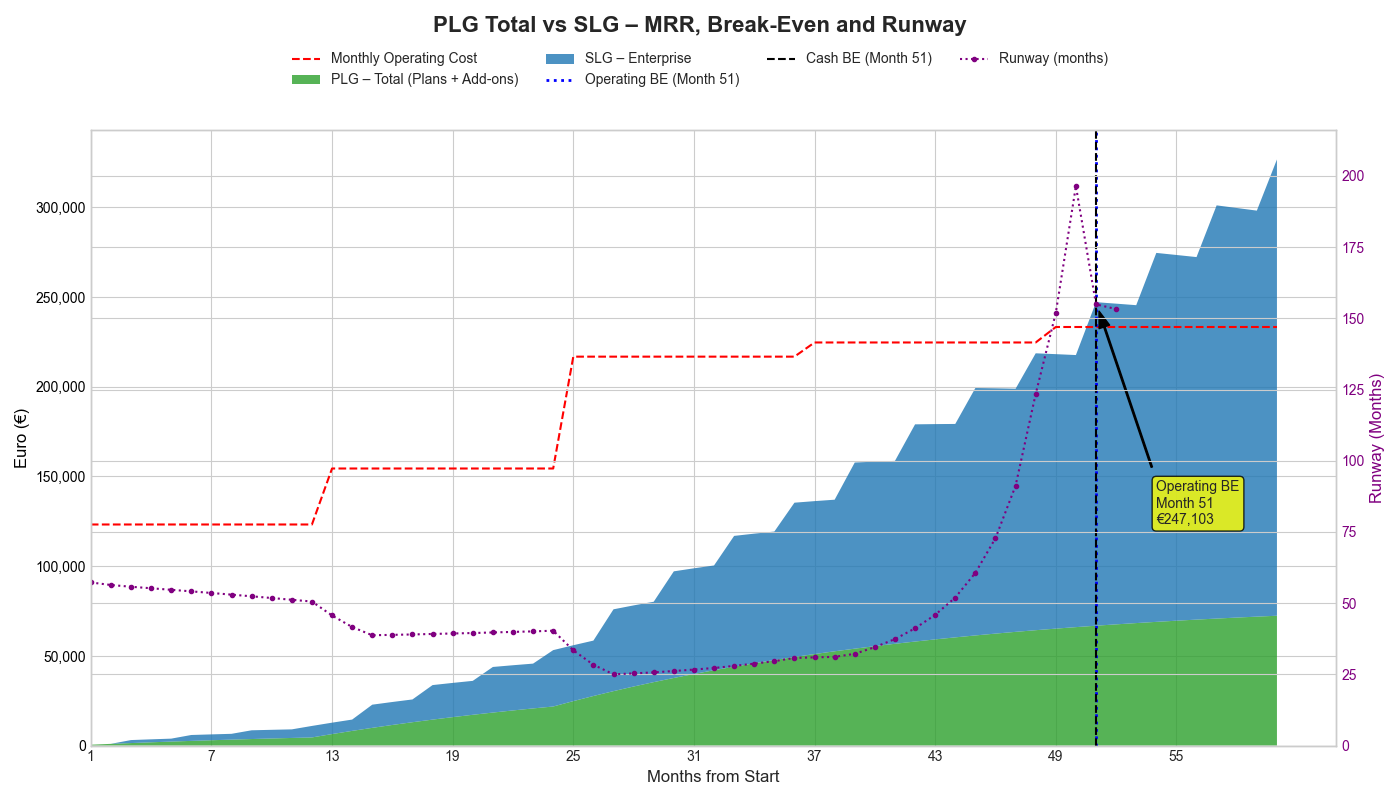
\includegraphics[width=\textwidth]{financial_projection.png}
    \caption{Break-even analysis: PLG vs. SLG MRR, monthly costs, and runway.}
    \label{fig:break_even_analysis}
\end{figure} 
\subsection{Break-even Analysis: Chart Interpretation}

\paragraph{Legend (quick read)}
\begin{itemize}
  \item \textbf{Green (PLG -- Plans + Add-ons):} self-service recurring revenue.
  \item \textbf{Blue (SLG -- Enterprise):} enterprise recurring revenue; grows in quarterly ``steps'' because annual deals are smoothed across quarters.
  \item \textbf{Red dashed:} monthly operating cost (with prudential uplifts), rising in yearly steps.
  \item \textbf{Purple dotted:} runway (months), computed as cash divided by the 3-month moving average burn.
  \item \textbf{Vertical lines:} operational break-even (blue, month~51) and cash break-even (black, month~51).
\end{itemize}

In the first three years the chart shows a patient build. The green PLG area rises steadily as monthly sign-ups compound (after churn) and add-ons add incremental MRR. The blue SLG area climbs in visible quarterly steps when enterprise contracts are booked. Costs move in blocks: each new year adds planned capacity (teams, infra, G\&A with uplifts), so the red line jumps and then stays flat until the next step.

These dynamics match the year-end figures. At the end of year~1, costs are \textbf{€123{,}212}/month versus \textbf{€10{,}948}/month of recurring MRR (loss \textbf{€112{,}149}/month, cash \textbf{€5{,}740{,}147}, runway \textbf{50.6} months). By year~2: \textbf{€154{,}413} vs.\ \textbf{€53{,}194} (loss \textbf{€100{,}855}/month), cash \textbf{€4{,}282{,}549}, runway \textbf{40.3} months. By year~3: \textbf{€216{,}746} vs.\ \textbf{€135{,}360} (loss \textbf{€80{,}631}/month), cash \textbf{€2{,}239{,}361}, runway \textbf{30.8} months. The curve of revenues clearly closes the gap to costs while cash remains controlled: the \textbf{minimum observed runway is 25.0 months} and the \textbf{peak monthly burn} is \textbf{€160{,}442}.

In year~4 the gap narrows decisively. The larger SLG steps make the blue area expand faster and the stack (PLG+SLG) nearly meets the cost line. Year-end: costs \textbf{€224{,}646}/month versus recurring MRR \textbf{€218{,}614}/month (total revenue \textbf{€219{,}615}/month), a near-flat loss of \textbf{€5{,}031}/month, cash \textbf{€2{,}239{,}361}. The purple runway line starts to spike because the moving-average burn approaches zero.

Break-even arrives in \textbf{month 51}. At that point \textbf{recurring MRR is €247{,}103} against \textbf{€233{,}271} of costs (operational BE), and \textbf{total revenue €248{,}159} exceeds costs (cash BE). To get there the model \textbf{burns €4{,}939{,}370} in total, with a \textbf{minimum cash} of \textbf{€2{,}234{,}573} that also represents the \textbf{reserve at BE (30.9\% of the round)}. By the end of year~5, recurring MRR reaches \textbf{€326{,}645}/month ($\approx$ \textbf{€3.92M ARR}), monthly profit is \textbf{€94{,}565}, cash is \textbf{€2{,}673{,}539}, and the runway becomes effectively infinite.

\paragraph{Takeaway}
The chart makes three things obvious:
\begin{enumerate}
\item \emph{who pushes what} PLG builds the base, SLG closes the gap
\item \emph{why costs jump} deliberate capacity steps with prudential uplifts
\item \emph{how cash stays protected} runway never collapses (min 25.0 months) and accelerates as the revenue stack overtakes costs, exactly as the printed metrics report.
\end{enumerate}

\begin{table}[H]
\centering
\caption{Financial Projection Summary (Year-End)}
\label{tab:financial_summary}
\resizebox{\textwidth}{!}{
\begin{tabular}{lrrrrrrr}
\toprule
\textbf{Year End} & \textbf{Monthly Cost (€)} & \textbf{Recurring MRR (€)} & \textbf{Store Revenue (€)} & \textbf{Total Revenue (€)} & \textbf{Monthly P/L (€)} & \textbf{Cash Balance (€)} & \textbf{Runway (months)} \\
\midrule
Year 1 & 123,212 & 10,948 & 116 & 11,064 & -112,149 & 5,740,147 & 50.6 \\
Year 2 & 154,413 & 53,194 & 364 & 53,558 & -100,855 & 4,282,549 & 40.3 \\
Year 3 & 216,746 & 135,360 & 755 & 136,115 & -80,631 & 2,823,198 & 30.8 \\
Year 4 & 224,646 & 218,614 & 1,001 & 219,615 & -5,031 & 2,239,361 & 123.5 \\
Year 5 & 233,271 & 326,645 & 1,191 & 327,836 & 94,565 & 2,673,539 & Profitable \\
\bottomrule
\end{tabular}
}
\end{table}

\begin{table}[H]
\centering
\caption{Key Financial Metrics}
\label{tab:financial_metrics}
\resizebox{\textwidth}{!}{%
\begin{tabular}{ll}
\toprule
\textbf{Metric} & \textbf{Value} \\
\midrule
Operating break-even & Month 51 (Year 5): Recurring MRR €247,103 $\geq$ Costs €233,271 \\
Break-even & Month 51 (Year 5): Total Revenue €248,159 $\geq$ Costs €233,271 \\
Capital burned until cash BE & €4,939,370 \\
Monthly peak burn & €160,422 \\
Minimum cash in period & €2,210,630 (30.9\% of round) \\
Minimum runway (3-month MA) & 25.0 months \\
\bottomrule
\end{tabular}
}
\end{table}

\newpage
\section{Why CNY 59{,}829{,}055 is the right amount}

We request \textbf{CNY 59{,}829{,}055} ($\approx€7.15\text{M}$) because this is exactly the amount of capital that, in our \emph{conservative} scenario, takes the company to \textbf{operational and cash break-even in month~51} without forcing growth and while preserving a concrete safety margin. The simulation results are explicit: \textbf{cumulative burn to cash break-even = €4{,}939{,}370}, \textbf{cash on hand at break-even = €2{,}210{,}630} (i.e., \textbf{30.9\%} of the round), \textbf{minimum runway along the path = 25.0 months} (3-month moving average), and \textbf{peak monthly burn = €160{,}422}. We are asking for the amount the model shows as \emph{necessary and sufficient} to reach break-even with a structural contingency buffer.

The plan is built to be resilient: costs are not ``bare-bones'' but \textbf{prudentially uplifted} by category (infrastructure, G\&A, PLG, SLG, R\&D, management) to capture recurring items that are often underestimated (enterprise support, audits, legal, recruiting, monitoring). In addition, the model introduces \textbf{automatic guardrails}: if runway drops below 12 months, \textbf{discretionary costs are cut by 10\%} the following month; below 9 months, \textbf{paid PLG acquisitions are damped} (multiplier 0.7). These are operational rules encoded in the model, not promises. In practice, the downside is protected by mechanisms that trigger on their own.

On the revenue side, we clearly separate \textbf{PLG} (plans + add-ons) and \textbf{SLG} (enterprise). This is not cosmetic: it lets us see, month by month, where spend levers return more and rebalance without ideology. With this mix and current prices, \textbf{operational break-even} arrives in \textbf{month~51} with \textbf{recurring MRR of €247{,}103} against \textbf{monthly costs of €233{,}271}; in the same month, \textbf{cash break-even} is achieved because \textbf{total revenue (€248{,}159)} exceeds costs. By the end of year $\sim 5$, recurring MRR reaches \textbf{€326{,}645} ($\approx$ \textbf{€3.92M ARR}). In terms of capital efficiency, the \textbf{implicit burn multiple} (burn to break-even $\div$ ARR at break-even) is \textbf{~1.66x}, consistent with a conservative product+go-to-market build and with costs already uplifted credibly.

Why, then, \emph{this} amount and not less? With less capital, the model would trigger guardrails more frequently, creating operational stop-and-go (cuts/cooling periods) that stretch timelines and raise opportunity cost precisely when continuity matters most. Why not more? Because beyond this threshold the bottleneck is not budget but \textbf{channel absorption} and the natural cadence of enterprise delivery; extra cash today would increase dilution without improving outcomes relative to the model.

\textbf{Use of proceeds} remains anchored to the very categories in the simulation and their uplifts: product/R\&D (hardening, observability, security), infrastructure \& enterprise support, SLG (account, solutions/POC), PLG (content/SDK/community), partner enablement, G\&A \& compliance, management. We are not opening new spend lines: we are funding what the model already measures month by month. 

Finally, the \textbf{risk profile} is readable. Minimum runway does not fall below \textbf{25.0 months}, guardrails limit cash erosion when needed, and the \textbf{30.9\%} buffer at break-even provides headroom against procurement delays, infra/compliance spend variability, or FX moves. At the same time, the PLG/SLG separation makes it straightforward—even ex post—to show that capital allocation followed realized returns rather than a one-size-fits-all plan.

\textbf{In short:} \textbf{CNY 59{,}829{,}055} fully finances the conservative path to break-even, with sufficient buffer and automated cost discipline. It is a proportional, defensible, and—above all—\textbf{replicable} ask: investors can verify month by month that model metrics remain under control and that cash tracks the expected trajectory.

\subsection{Strategic Buffer Rationale: Navigating the AI Orchestration Frontier}
The 30.9\% capital reserve at break-even (€2.21M) represents a deliberate strategic allocation for navigating the unprecedented velocity of change in the AI orchestration market. Unlike traditional SaaS sectors where product-market fit follows predictable patterns, the AI infrastructure landscape is experiencing fundamental shifts every 3-6 months—from new LLM architectures to emerging orchestration standards like MCP. This buffer enables IntellyHub to execute rapid strategic pivots without compromising runway: whether adapting to a breakthrough in autonomous agent capabilities, integrating game-changing models that didn't exist at planning time, or shifting focus between PLG and SLG channels based on real market response. Historical precedent from successful AI infrastructure companies (Weights \& Biases, Hugging Face) demonstrates that winners in this space required 2-3 significant pivots before achieving sustainable growth—each consuming 15-20\% of available capital. Our reserve ensures we can execute at least one major strategic realignment while maintaining 12+ months of operational runway, transforming what would be existential threats into competitive advantages. This is not excess capital; it's calculated optionality insurance in a market where the only certainty is radical change, and where the ability to pivot faster than competitors—while they scramble for emergency funding—becomes the decisive factor between market leadership and obsolescence.

\newpage
\section{Go-to-Market Strategy}
% Come raggiungerai i tuoi clienti?

IntellyHub's Go-to-Market (GTM) strategy is based on a hybrid model that combines two growth engines:
\begin{enumerate}
    \item \textbf{Product-Led Growth (PLG) for SaaS:} We leverage the superiority of the product, a Free Tier, and the Automation Store to attract, activate, and convert users in a scalable, bottom-up fashion.
    \item \textbf{Sales-Led Growth (SLG) for On-Premise \& Enterprise:} We use a targeted, consultative sales approach to win large customers with complex security and governance needs.
\end{enumerate}
These two engines are designed to be mutually reinforcing: the success of the PLG motion generates leads and brand awareness for the sales team.

% --- Strategic Objectives ---
\subsection{Strategic Objectives (3-Year Horizon)}
\begin{itemize}
    \item \textbf{Positioning:} To become a leading platform for orchestrating complex automations and AI workflows for modern technical teams.
    \item \textbf{Adoption:} To achieve critical mass of active users and a vibrant community around the plugin ecosystem and the automation store.
    \item \textbf{Revenue:} To build a sustainable business model with significant Annual Recurring Revenue (ARR), driven by both SaaS subscriptions and enterprise on-premise contracts.
\end{itemize}

% --- YEAR 1 ---
\subsection{Year 1: Foundation \& Market Validation}
\textbf{Main Focus:} Winning over early adopters, validating product-market fit, and securing the first key reference customers (both SaaS and On-Premise). In this phase, many activities are manual and "do not scale."

\newpage
\begin{table}[H]
\centering
\resizebox{\textwidth}{!}{
\begin{tabularx}{\textwidth}{L L L} 
\toprule
\textbf{Key Channels} & \textbf{Concrete Actions} & \textbf{Success KPIs} \\

\midrule
\textbf{Product-Led Growth (PLG)} & 
\textbf{Niche Launch:} Present IntellyHub on platforms like Product Hunt, Hacker News, and relevant technical subreddits (e.g., r/devops, r/kubernetes).\newline\newline
\textbf{Automation Store:} Populate the store with 20-30 high-quality official templates that solve real, painful problems.
&
\textbf{Activation Rate:} >25\% (users running their first automation within 7 days).\newline\newline
\textbf{1-Month Retention:} >15\% (users returning after 4 weeks).
\\
\addlinespace

\textbf{Technical Content Marketing} & 
\textbf{Blog \& Tutorials:} Publish 2-4 in-depth technical articles per month showcasing how to solve specific problems with IntellyHub.\newline\newline
\textbf{Video Content:} Create concise video tutorials.
&
\textbf{Qualified Traffic:} Number of site visits from organic and referral channels.\newline\newline
\textbf{Visitor-to-Signup Rate:} >2\%.
\\
\addlinespace

\textbf{Community Building} &
\textbf{Discord/Slack Channel:} Establish a central hub for early users.\newline\newline
\textbf{Founder-led Support:} Personally answer every question and feedback request to build a strong rapport.
&
\textbf{Community Engagement:} Weekly active members, peer-to-peer support interactions.\newline\newline
\textbf{Qualitative Feedback:} Minimum of 5 in-depth user interviews per month.
\\
\addlinespace

\textbf{Founder-Led Sales (On-Premise)} &
\textbf{Leverage Network:} Founders personally manage the first 3-5 sales processes with target companies from their own network.\newline\newline
\textbf{Proof of Concept (POC):} Focus on the success of a few high-value POCs.
&
\textbf{POCs Initiated:} 3-5 throughout the year.\newline\newline
\textbf{On-Premise Contracts Signed:} 1-2 key reference customers.
\\
\bottomrule
\end{tabularx}
}
\end{table}


% --- YEAR 2 ---
\newpage
\subsection{Year 2: Expansion \& Building a Repeatable Growth Engine}
\textbf{Main Focus:} Transforming initial value into scalable, repeatable processes. Optimizing what worked in Year 1 and building the foundation of a commercial team.

\begin{table}[H]
\small
\centering
\resizebox{\textwidth}{!}{
\begin{tabularx}{\textwidth}{L L L}
\toprule
\textbf{Key Channels} & \textbf{Concrete Actions} & \textbf{Success KPIs} \\
\midrule
\textbf{PLG Optimization} &

\textbf{Funnel Analysis:} Use analytics tools to identify and remove friction points in the user journey from signup to paid conversion.
\textbf{Guided Onboarding:} Implement an in-app onboarding experience that guides new users to their "Aha!" moment.
&

\textbf{Free-to-Paid Conversion Rate:} >3\%.
\textbf{MRR Growth Rate:} Consistent month-over-month growth.
\\
\addlinespace
\textbf{Ecosystem Partnerships} &

\textbf{Strategic Integrations:} Actively develop plugins for 2-3 complementary tech platforms with a similar user base.
\textbf{Co-Marketing:} Launch joint marketing campaigns with partners (webinars, blog posts).
&

\textbf{Partner-Sourced Leads.}
\textbf{Downloads of Partner Plugins.}
\\
\addlinespace
\textbf{Initial Sales Team} &

\textbf{First Hires:} Hire another Account Executives to handle inbound leads and begin targeted outbound prospecting.
\textbf{Sales Playbook:} Formalize the sales process based on lessons from the founder-led sales phase.
&

\textbf{Qualified Demos per Month.}
\textbf{Average Sales Cycle Length (On-Premise).}
\\
\bottomrule
\end{tabularx}
}
\end{table}

\newpage
% --- YEAR 3 ---
\subsection{Year 3: Scaling \& Segment Leadership}
\textbf{Main Focus:} Accelerating growth, dominating the technical team niche, and establishing IntellyHub as a thought leader in the AI orchestration market.

\begin{table}[H]
\centering
\resizebox{\textwidth}{!}{
\begin{tabularx}{\textwidth}{L L L}
\toprule
\textbf{Key Channels} & \textbf{Concrete Actions} & \textbf{Success KPIs} \\
\midrule
\textbf{Sales Scalability} &

\textbf{Team Expansion:} Grow the sales team to cover different geographies or industry verticals.
\textbf{Indirect Channels:} Begin exploring partnerships with System Integrators and Resellers.
&

\textbf{Annual Recurring Revenue (ARR) Growth.}
\textbf{Customer Acquisition Cost (CAC) and LTV/CAC Ratio.}
\\
\addlinespace
\textbf{Brand Marketing} &

\textbf{Thought Leadership:} Publish industry reports based on aggregated platform data.
\textbf{Sponsorships:} Sponsor key conferences and podcasts in the DevOps and AI space.
&

\textbf{Mentions in Industry Press.}
\textbf{Growth in Direct \& Branded Traffic.}
\\
\addlinespace
\textbf{Network Effect} &

\textbf{Open the Store:} Open the Automation Store and Plugin Marketplace to external contributions certificates partners.
\textbf{Developer Program:} Launch a formal Developer Relations (DevRel) program.
&

\textbf{Number of Community-Created Plugins/Templates.}
\textbf{Net Revenue Retention (NRR):} >110\%.
\\
\bottomrule
\end{tabularx}
}
\end{table}

\clearpage
\section{Operations Plan}
% Come funzionerà l'azienda giorno per giorno.
\subsection{Introduction}
This document outlines the operational plan to execute IntellyHub's development and go-to-market strategy. The plan is aligned with the phases of the Product Development Roadmap and describes the key activities for each functional area of the company.

% --- PHASE 1 ---
\subsection{Phase 1: Foundation and Validation (Quarters 1-2)}
\textbf{Strategic Objective:} To transform the prototype into a stable and secure MVP, acquire the first early adopters, and \textbf{validate the core product and pricing model hypotheses through a targeted partnership program.}

\subsubsection{Product Development \& Engineering}
\begin{itemize}[leftmargin=*]
    \item \textbf{Q1:}
    \begin{itemize}
        \item \textbf{Stabilization:} Complete the test suite (unit, integration) to ensure the reliability of the core engine.
        \item \textbf{Plugin:} Finalize and document the internal system to enable standardized plugin development.
        \item \textbf{UI/UX:} Refine the hybrid IDE interface to resolve any synchronization issues and improve the user experience.
        \item \textbf{On-Premise:} Develop and test the on-premise version of the platform for enterprise customers.
    \end{itemize}
    \item \textbf{Q2:}
    \begin{itemize}
        \item \textbf{Authentication:} Implement a robust user management and authentication system.
        \item \textbf{Onboarding:} Develop a guided onboarding wizard for new users.
        \item \textbf{Store (v1):} Create the API and UI for the first version of the Automation Store (read-only).
    \end{itemize}
\end{itemize}

\subsubsection{Go-to-Market (Marketing \& Sales)}
\begin{itemize}[leftmargin=*]
    \item \textbf{Q1-Q2:}
    \begin{itemize}
        \item \textbf{Vertical Strategy:} Define a detailed Ideal Customer Profile (ICP) within an \textit{initial vertical niche} (e.g., BioTech/Scientific Research, based on the user case of Esplorado).
        \item \textbf{(New) Design Partner Program:} Launch an exclusive program for 3-5 selected companies in the target vertical. Offer early access and direct support in exchange for continuous feedback and a potential preliminary contract.
    \end{itemize}
    \item \textbf{Q3-Q4:}
    \begin{itemize}
        \item \textbf{Niche Launch:} Execute the launch on Product Hunt, Hacker News, and relevant channels, with communication focused on the chosen vertical.
        \item \textbf{Feedback Collection:} Gather structured feedback from both Free Tier users and, with priority, from Design Partners.
    \end{itemize}
\end{itemize}

\subsubsection{Community \& Ecosystem Management}
\begin{itemize}[leftmargin=*]
    \item \textbf{Q1-Q2:}
    \begin{itemize}
        \item \textbf{Targeted Plugin Development:} Develop and document the first "official" plugins, giving \textit{priority to those most relevant to the target vertical}.
    \end{itemize}
    \item \textbf{Q3-Q4:}
    \begin{itemize}
        \item \textbf{Community Creation:} Launch the official Discord/Slack server.
        \item \textbf{Engagement:} Founders and the development team will actively participate to answer questions and create a welcoming environment.
    \end{itemize}
\end{itemize}

\subsubsection{General \& Corporate Operations}
\begin{itemize}[leftmargin=*]
    \item \textbf{Q1-Q2:}
    \begin{itemize}
        \item \textbf{Legal and Administrative Setup:} Finalize the corporate structure, open bank accounts.
        \item \textbf{(New) Partner Contracting:} Prepare the agreements for the "Design Partner Program."
    \end{itemize}
    \item \textbf{Q3-Q4:}
    \begin{itemize}
        \item \textbf{Terms of Service Definition:} Write and publish the Terms of Service and Privacy Policy for the Free Tier launch.
    \end{itemize}
\end{itemize}

\clearpage

% --- PHASE 2 ---
\subsection{Phase 2: Expansion and Growth (Quarters 3-4)}
\textbf{Strategic Objective:} To scale user acquisition, expand the ecosystem, and implement the necessary enterprise features for monetization, based on the data validated in Phase 1.

\subsubsection{Product Development \& Engineering}
\begin{itemize}[leftmargin=*]
    \item \textbf{Q5-Q6:}
    \begin{itemize}
        \item \textbf{Security:} Implement a secrets management system for credentials.
        \item \textbf{Versioning:} Add history and rollback functionality for automations.
    \end{itemize}
    \item \textbf{Q7-Q8:}
    \begin{itemize}
        \item \textbf{Observability:} Develop the first version of the data platform for flow performance metrics.
        \item \textbf{Improve Dashboards:} Create a user interface for visualizing flows.
        \item \textbf{Proactive AI:} Implement basic "auto-healing" features based on flow performance data.
    \end{itemize}
\end{itemize}

\subsubsection{Go-to-Market (Marketing \& Sales)}
\begin{itemize}[leftmargin=*]
    \item \textbf{Q5-Q6:}
    \begin{itemize}
        \item \textbf{Vertical Content Marketing:} Scale the production of content (case studies based on Design Partners, articles) focused on the chosen vertical.
        \item \textbf{Hiring:} Begin the recruitment process for the first Developer Advocate.
    \end{itemize}
    \item \textbf{Q7-Q8:}
    \begin{itemize}
        \item \textbf{Paid Plans Launch:} Finalize pricing (validated with Design Partners) and officially launch the Pro and Enterprise plans.
        \item \textbf{Sales Playbook (v1):} Begin documenting the sales process for enterprise customers.
    \end{itemize}
\end{itemize}

\clearpage

% --- PHASE 3 ---
\subsection{Phase 3: Leadership and Innovation (Quarters 5-6)}
\textbf{Strategic Objective:} To establish market leadership, create a network effect through the community, and **leverage data to build an insurmountable competitive advantage.**

\subsubsection{Product Development \& Engineering}
\begin{itemize}[leftmargin=*]
    \item \textbf{Q9-Q10:}
    \begin{itemize}
        \item \textbf{Store Opening:} Open the Store to allow content submission from the community.
        \item \textbf{Moderation:} Implement internal tools for the review and validation of external contributions.
    \end{itemize}
    \item \textbf{Q11-Q12:}
    \begin{itemize}
        \item \textbf{(Revised) Data Platform \& Observability:} Develop the system for collecting and aggregating flow performance metrics, with the strategic goal of \textbf{building a "Data Moat"}.
        \item \textbf{Analytics Dashboard:} Create the user interface for visualizing analytics.
        \item \textbf{Proactive AI:} Improve "auto-healing" and proactive optimization features, \textbf{trained on aggregated platform data}.
    \end{itemize}
\end{itemize}

\subsubsection{Go-to-Market (Marketing \& Sales)}
\begin{itemize}[leftmargin=*]
    \item \textbf{Q9-Q10:}
    \begin{itemize}
        \item \textbf{Sales Team Scaling:} Hire additional Account Executives to cover specific markets or verticals.
        \item \textbf{Thought Leadership:} Begin publishing reports and analyses based on platform usage data.
    \end{itemize}
    \item \textbf{Q11-Q12:}
    \begin{itemize}
        \item \textbf{Brand Marketing:} Increase investment in brand awareness activities (sponsorships, events).
    \end{itemize}
\end{itemize}

\newpage
\section{Risk Analysis}
\subsection{Market Risks}
\textit{Risks related to the market, competition, and customer adoption.}

\begin{table}[H]
\centering
\begin{tabularx}{\textwidth}{@{}lL@{}}
\toprule
\textbf{Risk} & \textbf{Description} \\
\midrule
\textbf{Competition from the "Status Quo"} & Our biggest competitor is not another platform, but the inertia of developers using custom Python scripts. Their familiarity and the perceived zero initial cost make it a significant hurdle to overcome. \\
\addlinespace
\textbf{Slow Enterprise Adoption Cycle} & The on-premise and enterprise sales model is crucial for high-value contracts, but it is characterized by long sales cycles (6-12+ months) and complex proof-of-concept (POC) phases. A delay in closing the first key enterprise deals could significantly impact revenue projections. \\
\addlinespace
\textbf{AI Technology Shift} & Our AI is currently positioned as a "copilot." A rapid technological leap by a competitor towards a truly autonomous AI agent that is "good enough" could make our more controlled, structured approach seem less innovative. \\
\bottomrule
\end{tabularx}
\end{table}

\newpage
\subsection{Operational Risks}
\textit{Risks related to technology, personnel, and execution.}

\begin{table}[H]
\centering
\begin{tabularx}{\textwidth}{@{}lL@{}}
\toprule
\textbf{Risk} & \textbf{Description} \\
\midrule
\textbf{Team Execution \& Key-Person Risk} & The plan relies on hiring a small number of highly specialized individuals. The success of the project is highly dependent on this core team's ability to execute across product, infrastructure, and sales. The departure of a key member could cause significant delays. \\
\addlinespace
\textbf{Technological Complexity} & The tech stack (Kubernetes, multi-step AI pipelines, hybrid IDE) is extremely powerful but also complex to maintain and evolve. Bugs, security vulnerabilities, or performance bottlenecks in this complex system can be difficult and costly to resolve. \\
\addlinespace
\textbf{Hybrid Technology Risk (IDE/YAML Sync)} & Maintaining a perfect, real-time, bidirectional synchronization between the complex visual IDE and the textual YAML representation is technically demanding. It is a potential source of subtle and hard-to-debug bugs that could affect user trust. \\
\addlinespace
\textbf{Ecosystem Quality Control} & The value of the Automation Store and Plugin Marketplace is a double-edged sword. Low-quality, insecure, or poorly maintained community contributions could damage user trust and the platform's reputation. \\
\bottomrule
\end{tabularx}
\end{table}

\newpage
\subsection{Financial Risks}
\textit{Risks related to cash flow, funding, and financial sustainability.}

\begin{table}[H]
\centering
\begin{tabularx}{\textwidth}{@{}lL@{}}
\toprule
\textbf{Risk} & \textbf{Description} \\
\midrule
\textbf{High Initial Burn Rate} & The aggressive hiring plan results in a high monthly operational cost  before significant revenue is generated. This creates immense pressure to achieve product-market fit and generate revenue quickly. \\
\addlinespace
\textbf{Funding Dependency} & The business model is not designed for short-term profitability. Failure to meet the growth KPIs expected by investors is an existential threat. \\
\addlinespace
\textbf{Pricing Model Validation} & The proposed value metrics (executions, active automations) are logical but untested. An incorrect pricing model could lead to customer friction (if too expensive) or leave significant revenue on the table (if too cheap). \\
\bottomrule
\end{tabularx}
\end{table}

\newpage
\subsection{Mitigation Strategies}
\textit{Concrete actions to address and reduce the identified risks.}

\begin{table}[H]
\centering
\begin{tabularx}{\textwidth}{@{}lL@{}}
\toprule
\textbf{Risk Category} & \textbf{Mitigation Strategy} \\
\midrule
\textbf{Market Risks} & 
\textbf{Positioning \& Education:} Focus marketing not on replacing a single script, but on eliminating the long-term chaos of managing \textit{many} scripts. Use case studies like "Esplorado" to provide undeniable proof of value. \newline\newline
\textbf{Hybrid GTM:} Run the PLG (SaaS) and SLG (On-premise) motions in parallel. Use the faster feedback loop from the PLG side to refine the product and messaging for the slower enterprise sales cycle. \newline\newline
\textbf{Strategic AI Roadmap:} Position the current AI as the pragmatic, secure, and reliable choice for production environments. Frame the roadmap as an evolution towards more autonomous capabilities, building on the robust foundation we have today. \\
\addlinespace
\textbf{Operational Risks} & 
\textbf{Documentation \& Cross-Training:} Invest heavily in internal documentation from day one. Implement a culture of knowledge sharing and pair programming to reduce dependency on single individuals. \newline\newline
\textbf{Invest in Observability \& Testing:} Dedicate resources to a robust automated testing suite and integrate an APM (Application Performance Monitoring) tool early on to proactively identify and resolve issues. The test suite specifically covers the IDE/YAML sync logic. \newline\newline
\textbf{Curated Ecosystem:} Initially, the Store will only feature "Official" and "Verified Partner" plugins. Implement a clear and rigorous review process for all future community submissions, including automated security scans and quality checks. \\
\addlinespace
\textbf{Financial Risks} & 
\textbf{Milestone-Based Spending:} Tie major increases in spending (especially on marketing and sales hires) to the achievement of specific, pre-defined milestones (e.g., reaching the first 10 paying customers, achieving a certain retention rate). \newline\newline
\textbf{Continuous Investor Relations:} Maintain a transparent and regular communication channel with current and potential future investors, sharing progress on KPIs to build confidence and streamline the next funding round. \newline\newline
\textbf{Pricing Iteration:} Launch with a simple, flexible pricing model. Engage directly with early customers to understand the value they are getting and be prepared to iterate on the pricing structure based on their feedback and usage data. \\
\bottomrule
\end{tabularx}
\end{table}

% \newpage
% \subsection{Product Screenshots}
% Screenshot, mockup o diagrammi del prodotto.

\newpage
% Aggiungi qui eventuali fonti, studi o articoli citati nel documento.
\begin{thebibliography}{99}
    \bibitem{AIMarket}
    Market.us, \textit{Automated Machine Learning Market Report}, Available at: \url{https://market.us/report/automated-machine-learning-market/}, March~2025.
    
    \bibitem{MLOpsMarket}
    MarketReserchFuture.com, \textit{Mlops Market Research Report: Information By Component (Service, Platform), By Deployment Mode (On-Premises, Cloud), By Organization Size (Large Enterprise, SME's), By Verticals (BFSI, Retail and e-Commerce, Government and Defense, Healthcare and Life science, Manufacturing, and Others) And By Region (North America, Europe, Asia-Pacific, And Rest Of The World) –Market Forecast Till 2034.}, Available at: \url{https://www.marketresearchfuture.com/reports/mlops-market-18849}, Agoust~2025.
    
    \bibitem{AIOrch}
    Market.us, \textit{AI Orchestration Platform Market Report (2024--2034 Forecast)}, February~2025.  
    Available at: \url{https://market.us/report/ai-orchestration-platform-market/}.

    \bibitem{GartnerAgentic}
    Reuters (reporting Gartner), \textit{Over 40\% of agentic AI projects will be scrapped by 2027 … by 2028, 33\% of enterprise software will include agentic AI and 15\% of decisions will be made autonomously,} June~25,~2025.  
    Available at: \url{https://www.reuters.com/business/over-40-agentic-ai-projects-will-be-scrapped-by-2027-gartner-says-2025-06-25/}.

    \bibitem{MLOpsMM}
    MarketsandMarkets Research, \textit{MLOps Market Size is Anticipated to Cross US\$5.9 Billion by 2027, growing at a CAGR of 41.0\%}, April~21,~2023.  
    Available at: \url{https://www.globenewswire.com/news-release/2023/04/21/2652028/0/en/MLOps-Market-Size-is-Anticipated-to-Cross-US-5-9-billion-by-2027-growing-at-a-CAGR-of-41-0-Report-by-MarketsandMarkets.html}.

    \bibitem{ModelOpsGV}
    Grand View Research, \textit{ModelOps Market Report}, 2025 edition.  
    Available at: \url{https://www.grandviewresearch.com/industry-analysis/modelops-market-report}.

    \bibitem{AIMLMarket}
    Market.us, \textit{Automated Machine Learning Market Report (2024--2034 Forecast)}, March~2025.  
    Available at: \url{https://market.us/report/automated-machine-learning-market/}.

    \bibitem{MLOpsMRF}
    MarketResearchFuture, \textit{MLOps Market Research Report (2024--2034 Forecast)}, August~2025.  
    Available at: \url{https://www.marketresearchfuture.com/reports/mlops-market-18849}.

    \bibitem{deloitte2020}
    Deloitte, \textit{Automation with the intelligent edge: A new frontier for a supercharged enterprise}, 2020. Available at: \url{https://www2.deloitte.com/us/en/insights/topics/talent/intelligent-automation-2020-survey-results.html}

    \bibitem{grandviewRPA}
    Grand View Research, \textit{Robotic Process Automation (RPA) Market Size, Share \& Trends Analysis Report}, 2024. Available at: \url{https://www.grandviewresearch.com/industry-analysis/robotic-process-automation-rpa-market}

    \bibitem{mckinseyAI2023}
    McKinsey \& Company, \textit{The state of AI in 2023: Generative AI’s breakout year}, August 1, 2023. Available at: \url{https://www.mckinsey.com/capabilities/quantumblack/our-insights/the-state-of-ai-in-2023-generative-ais-breakout-year}


    \bibitem{langchainGitHub}
    LangChain GitHub Repository. Available at: \url{https://github.com/langchain-ai/langchain}

    \bibitem{gartnerAIBarriers}
    Gartner, \textit{2 Barriers to AI Adoption}, November 2, 2021. Available at: \url{https://www.gartner.com/en/articles/2-barriers-to-ai-adoption}

    \bibitem{euAIAct}
    European Commission, \textit{Regulatory framework proposal on artificial intelligence}. Available at: \url{https://digital-strategy.ec.europa.eu/en/policies/regulatory-framework-ai}
    
    \bibitem{AIOrch}
    Market.us, \textit{AI Orchestration Platform Market Report (2024--2034 Forecast)}, February~2025. Available at: \url{https://market.us/report/ai-orchestration-platform-market/}.

    \bibitem{zapierApps}
    Zapier, \textit{Explore 6,000+ apps}. Available at: \url{https://zapier.com/apps}

    \bibitem{g2ZapierReviews}
    G2, \textit{Zapier Reviews}. Available at: \url{https://www.g2.com/products/zapier/reviews}

    \bibitem{zapierPricing}
    Zapier, \textit{Zapier Pricing Plans}. Available at: \url{https://zapier.com/pricing}


    \bibitem{zapierOpenAI}
    Zapier, \textit{OpenAI Integrations}. Available at: \url{https://zapier.com/apps/openai/integrations}

    \bibitem{g2MakeVsZapier}
    G2, \textit{Compare Make vs. Zapier}. Available at: \url{https://www.g2.com/compare/make-vs-zapier}


    \bibitem{autogenGitHub}
    Microsoft, \textit{AutoGen GitHub Repository}. Available at: \url{https://github.com/microsoft/autogen}

    \bibitem{crewaiGitHub}
    Joao Moura, \textit{CrewAI GitHub Repository}. Available at: \url{https://github.com/joaomdmoura/crewAI}

    \bibitem{langchainValuation}
    TechCrunch, \textit{AI infrastructure startup LangChain reportedly raises $100M at $1.1B valuation}, July 9, 2025. Available at: \url{https://siliconangle.com/2025/07/09/ai-infrastructure-startup-langchain-reportedly-raises-100m-1-1b-valuation/#:~:text=Artificial%20intelligence%20infrastructure%2C%20developer%20tools,on%20a%20%241.1%20billion%20valuation.}

    \bibitem{langchainIntegrations}
    LangChain Documentation, \textit{LangChain Integrations}. Available at: \url{https://python.langchain.com/docs/integrations/providers/}

    \bibitem{langchainCritique}
    Medium, \textit{Challenges \& Criticisms of LangChain}, March 3, 2025. Available at: \url{https://shashankguda.medium.com/challenges-criticisms-of-langchain-b26afcef94e7}

    \bibitem{mrfRPA}
    Market Research Future, \textit{Robotic Process Automation (RPA) Market Research Report Information By Process (Decision Support, Automated Solution, and Management Solution), By Operations (Rule-based, and Knowledge-based), By Industry (Manufacturing \& Logistics, and IT \& Telecommunication), and By Region (North America, Europe, Asia-Pacific, And Rest of the World) –Industry Size, Share and Forecast Till 2032}. Available at: \url{https://www.marketresearchfuture.com/reports/robotic-process-automation-market-2209}

    \bibitem{uipathGartner}
    UiPath, \textit{Gartner Magic Quadrant for RPA}, 2025. Available at:
    \url{https://www.uipath.com/resources/automation-analyst-reports/gartner-magic-quadrant-robotic-process-automation}

    \bibitem{awsSagemaker}
    Amazon AWS SageMaker, \textit{Amazon SageMaker}, Available at: \url{https://aws.amazon.com/sagemaker/}

    \bibitem{forresterRPAvsAI}
    Craig Le Clair, \textit{Will RPA Platforms Remain Relevant? AI Agents May Hold The Answer.}, Forrester, April 25, 2024. Available at: \url{https://www.forrester.com/blogs/will-rpa-platforms-remain-relevant-ai-agents-may-hold-the-answer/}

\end{thebibliography}


\end{document}
